\chapter*{第四部分:感知}
\markboth{总论}{总论}

\begin{figure}[htbp]
	\centering
	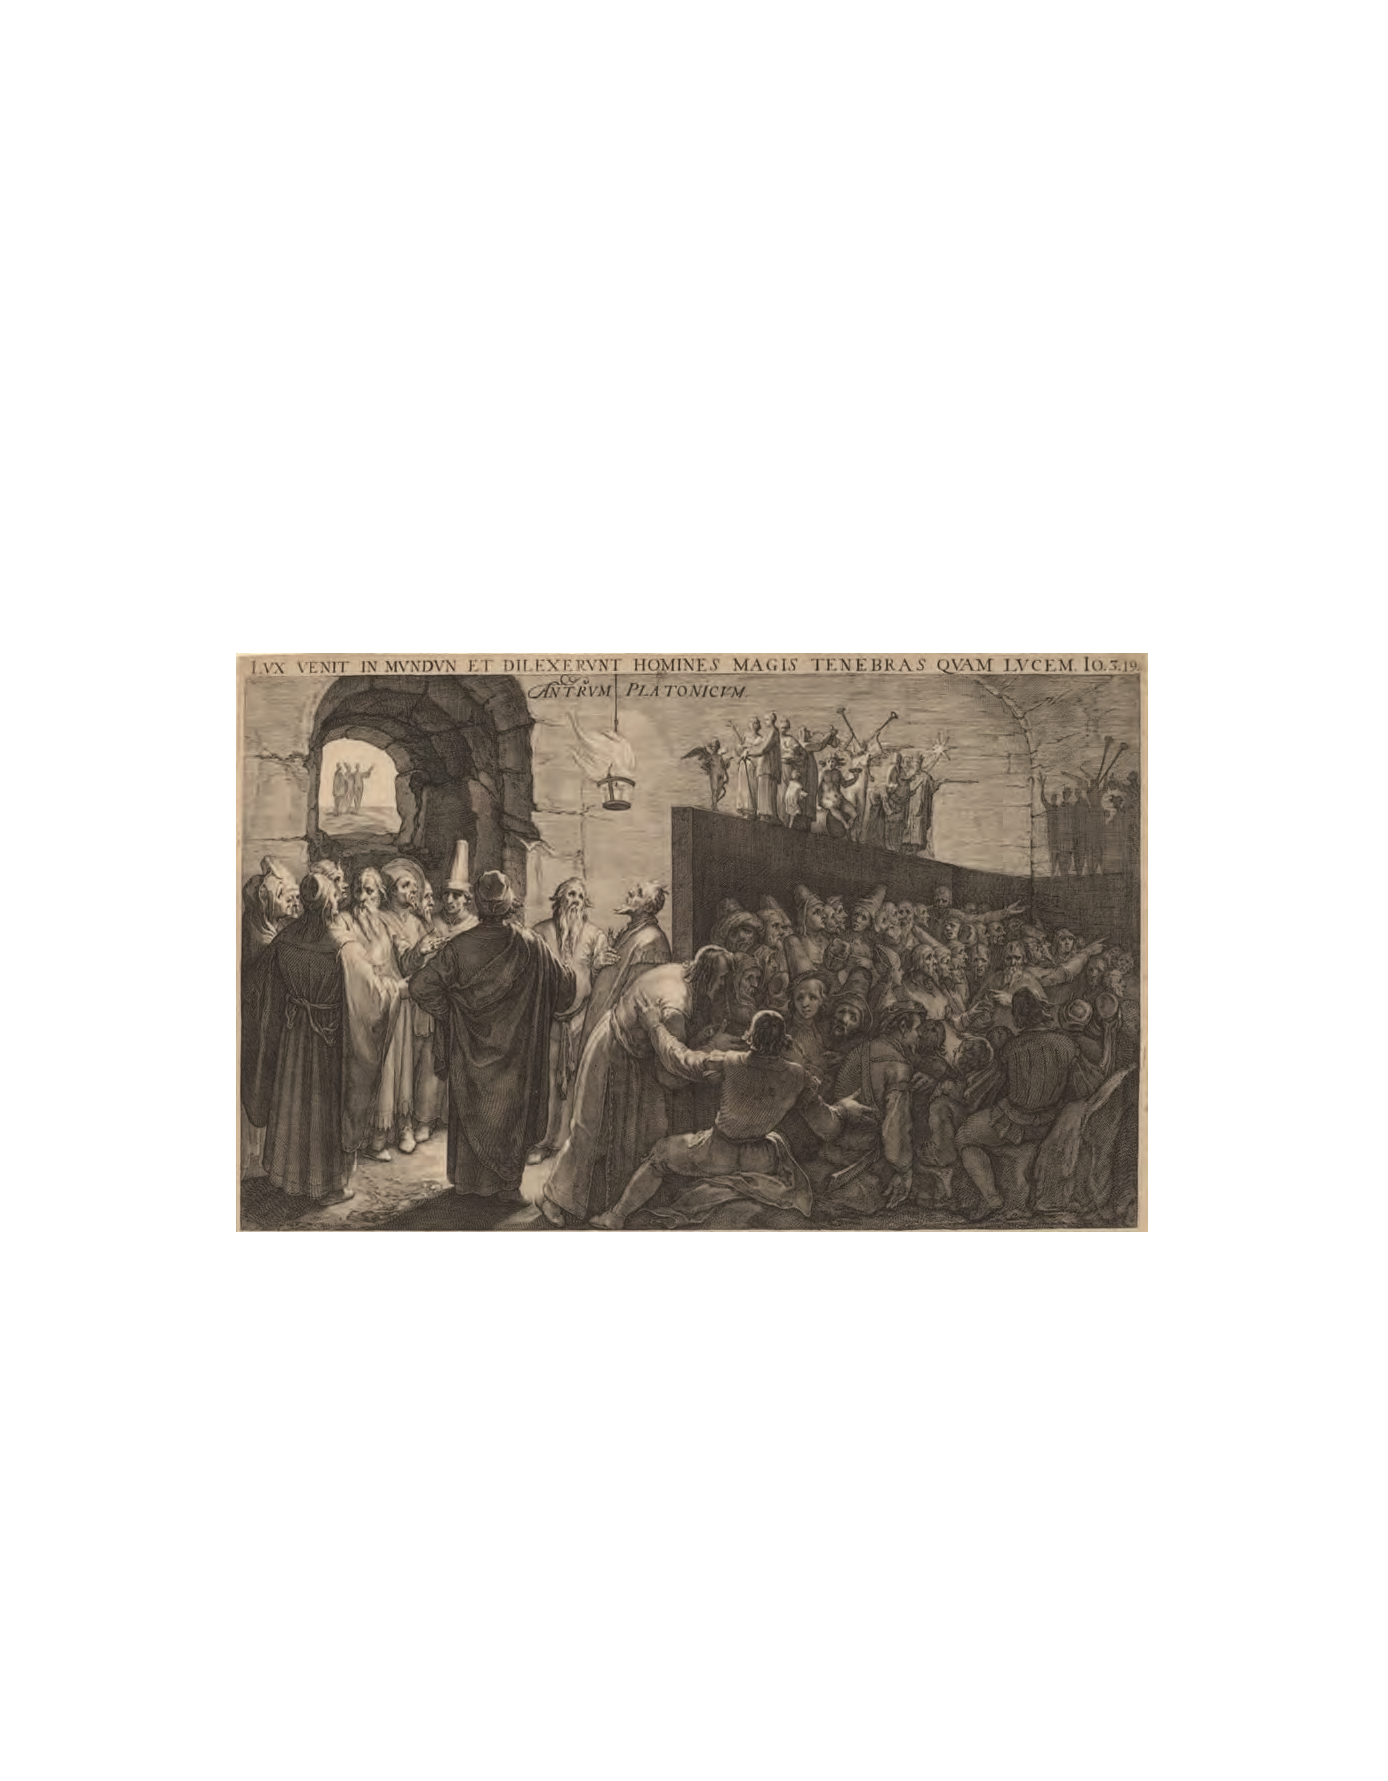
\includegraphics[width=0.9\linewidth]{chap17/fig_17_0}
	\caption{在柏拉图关于知识起源的《洞穴寓言》中,他对感知的建设性本质的早期见解为这一过程提供了启发性的隐喻。
		这个寓言以一群囚犯从未见过外面的世界为前提。
		他们的经验仅限于火灾前经过的物体投射在洞穴墙壁上的阴影。
		这些阴影的原因——甚至是它们是阴影的事实——囚犯们都不知道。
		尽管如此,随着时间的推移,这些阴影在囚犯的脑海中变得充满了意义。
		从隐喻的角度来说,阴影代表着短暂而不连贯的感觉。
		意义的分配代表了可理解感知的构建。
		翻墙的囚犯被释放,见证了更大的事业世界,他向仍被监禁的人报告了这一情况。
		在对这个古老故事的新颖隐喻中,这位归来的囚犯代表了现代神经科学的领域,揭示了我们对世界的模糊感觉和丰富的感知体验之间的关系。
		(柏拉图洞穴,1604年。Jan Pietersz Saenredam,以Cornelis Corneliz van Haarlem命名。国家美术馆,华盛顿特区)}
	\label{fig:17_0}
\end{figure}

我明白这个世界什么都不是:一个随意的、野蛮的敌意的机械混乱,我们愚蠢地把希望和恐惧强加在上面。
我终于明白,我是唯一存在的。
我看到,剩下的一切都只是推动我的东西,或者我盲目地反对的东西——就像所有不是我自己的东西都在盲目地推动一样。
我创造了整个宇宙,一眨眼…。
尽管如此,这一切还是会有结果的。


约翰·加德纳(John gardner)讲述了饱受折磨的怪物格伦德尔(Grendel)对生活的看法,这是一个令人心碎的故事,它抓住了感知体验的基本本质:这是一种我们自己强加的结构。
或者,正如格伦德尔敏锐地观察到的那样,“山脉就是我对它们的定义。”
格伦德尔被孤独所孤立和折磨,他看到的世界就像柏拉图洞穴中戴着镣铐的囚犯一样,在那里,人们只感觉到阴影,但这些阴影充满了意义、效用、能动性、美、欢乐和悲伤,通过建设性的感知过程:“我看到的,我用有用的东西激励……而我没有看到的,都是无用的,空虚的。”


就像从柏拉图洞穴逃脱去观察更大原因世界的囚犯,或者让格伦德尔充满另一个维度想法的无所不知的龙一样——“但龙,我的孩子,有一种完全不同的思维……我们从山顶看到:所有的时间,所有的空间”——现代神经科学承诺对感知体验有一种山顶理解,不仅仅是对我们从模糊的感觉中构建的东西的理解,还有我们是如何做到的,以及为了什么目的。


关于感知的这一部分提供了广阔的山顶景观。
对于每一种感官模式,这些章节都从研究环境刺激开始——光、声音、重力、触摸和化学物质——这些都是人类经验和世界知识的起源。
以分层的方式,各章调查了实现刺激检测和辨别的机制,用意义填充消逝感觉的感知过程,以及基于感知支持注意力、决策和行动的操作。


视觉——一种被人类充分理解和大量利用的感觉——通过光的特性获取信息。
从环境中的物体反射的光的波长和强度各不相同,并在空间和时间上波动,通过这些物理特性传递我们周围世界的证据。
将光能以图案图像的形式投射在视网膜上,通过专用的受体细胞将其转换为神经元信号。
这些图像的证据特性是由一组专门的神经元系统检测到的,这些系统感知对比的形式并将这些信息传达给大脑的其他部分。


类似地,听觉系统通过口语、音乐或环境声音引起的空气的简单压缩和稀薄来获取有关世界的信息。
这种感觉证据是通过一个由小鼓、杠杆、管和毛细胞组成的极其复杂的扩增系统检测到的,即使是以微小的数量和令人难以置信的精确时间,其可弯曲的立体纤毛将机械能转换为神经元信号。
类似的运动检测毛细胞为头部的平衡、加速和旋转的前庭感觉服务。


体感系统获取关于以压力、振动和温度的形式撞击身体的物理刺激的信息,在极端情况下,还会获取疼痛的信息,这可能是由触摸、皮肤在纹理表面上的运动或与热源的接触引起的。
嵌入皮肤、内脏和肌肉中的各种特殊检测神经元的外周神经末梢将这种机械能转换为神经元信号,这些信号通过脊髓和脑神经传递到大脑。


最后,味觉和嗅觉以食物、饮料和空气中分子的形式获取有关世界化学成分的信息。
在当今感官生物学最令人兴奋和发展最快的领域之一,我们现在知道有数百种嗅觉受体对空气中的分子具有独特的亲和力,这就是人类检测和辨别数量惊人且多样性气味的能力。


所有这些感受系统都充当过滤器,其特征是突出某些形式的信息并限制其他形式的信息的神经“感受场”。
这些选择性滤波器在不同的时间尺度上是可调的,可以增强对显著刺激的关注,并适应感官世界的统计数据。
这种灵活性适应了行为目标和环境条件的变化。


就像柏拉图洞穴中戴着镣铐的囚犯一样,我们的感官系统最初传达的是对感官输入的简单过滤表示,这些表示从根本上来说是模糊、嘈杂和不完整的。
他们一个人没有意义。
非常值得注意的是,我们的大脑使我们能够最终体验到这些感官信息,作为导致这些模式的环境对象和事件。
从感官证据世界到意义世界的建设性转变是感知的核心,长期以来一直是人类认知中最引人入胜的奥秘之一。
19世纪的英国哲学家约翰·斯图尔特·密尔(John Stuart Mill)写道,“感知反映了感知的永久可能性”,并在这样做的过程中,从短暂的感官事件中恢复了世界持久的结构和关系特性。


本节揭示了感知如何克服感官证据的变幻莫测,通过参考过去的知识来发展关于感觉原因的假设或推论。
这大部分是通过大脑皮层的机制发生的,在大脑皮层中,感觉信号在模态内部和模态之间以及与记忆存储的反馈都有联系。
就像一个侦探在记忆和背景的作用下观察犯罪现场一样,大脑皮层神经元的活动开始产生威廉·詹姆斯(WilliamJames)恰当地称之为“对可能事物的感知”。


随着这种知觉的转变,我们也能够识别我们熟悉的物体。
我们很容易以知觉恒常性和范畴知觉的形式概括相同或相似物体的不同感官表现,并将其与其他有意义的事件联系起来。
早晨咖啡研磨机的声音,情人香水的气味或她的脸,将我们的体验扩展到超越眼前的回忆和想象的领域。
本系列中的章节回顾了构成这些关联功能基础的大脑结构和计算,其中包括用于识别和解释复杂和行为重要对象(例如面部)的高度专业化的神经元系统。


对我们周围世界的感知体验是与这个世界进行有意义互动的先决条件。
决策是基于感官证据的积累来支持一种感知与另一种感知。
旋转木马上的是我的手提箱吗?
这是我们要转弯的地方吗?
那是瓦格纳的咏叹调还是施特劳斯的?
那是茉莉花的香味还是栀子的香味?
皮层神经元形成显着性图,它代表了这些感知决策在行为目标和奖励方面的结果,并相应地优先考虑行动。


感知通常被视为神经科学的一个独特的分支学科。我们越来越多地看到这种划分被打破。
随着监测和操纵大脑结构和功能以及揭示看似不同的大脑区域之间广泛的解剖和功能神经联系的新概念和实验方法的爆炸性增长,感知与其他大脑功能的关系学习,记忆,情绪,运动控制,语言,发育变得更加清晰。
因此,我们开始充分认识到大脑获取和解释信息的系统,以及意识和理解感知世界的系统是人类认知和行为的功能中心。



\chapter{感觉编码} \label{chap:chap17}

% 参考:https://www.dxy.cn/bbs/newweb/pc/post/40268362

我们的感官启发并赋予我们力量。 
通过感觉,我们根据过去的经验形成一幅直接且相关的世界图景以及我们在其中的位置,并为可能的未来做好准备。 
% 检测、识别、跟踪
感觉可以立即回答三个持续存在的基本问题:那里有东西吗? 它是什么? 有什么变化? 
为了回答这些问题,所有感觉系统都执行两个基本功能:检测和识别。 
因为我们的世界和我们对它的反应会随着时间而变化,所以感觉系统既可以在短期内优先反应和适应不断变化的刺激,也可以随着我们的需求和环境的变化学会修改我们对刺激的反应。


自古以来,人类就对感官体验的本质着迷。 
亚里士多德定义了五种感觉——视觉、听觉、触觉、味觉和嗅觉——每一种都与身体中特定的感觉器官相关联:眼睛、耳朵、皮肤、舌头和鼻子。 
疼痛不被认为是一种特定的感觉方式,而是一种灵魂的痛苦。 
直觉,通常被通俗地称为“第六感”,尚未被理解为依赖于经典感官系统的经验。 
今天,神经生物学家认为直觉是从以前的经验中得出的推论,因此是认知和感觉过程的结果。


在本章中,我们将考虑对所有感觉系统都通用的组织原则和编码机制。 
感觉信息被定义为源自刺激身体特定部位的受体细胞的神经活动。 
我们的感官包括经典的五种感官以及古人未认识到但对身体机能必不可少的各种形式:疼痛、瘙痒、温度和本体感觉(我们自己身体的姿势和运动)的躯体感觉; 
体内平衡所必需的内脏感觉(有意识和无意识); 
以及前庭平衡感(身体在重力场中的位置)和头部运动。


感觉丰富了所有生命,感觉处理的基本原理在整个脊椎动物进化过程中得到了保护。
每个感觉系统中的专门受体提供外部和内部世界的第一个神经表征,将特定类型的刺激能量转化为电信号(图~\ref{fig:17_1})。 
然后,所有感觉信息都通过代表刺激特定方面的动作电位序列传输到中枢神经系统。
这些信息集中流向大脑中涉及处理个人感觉、多感官整合和认知的区域。


\begin{figure}[htbp]
	\centering
	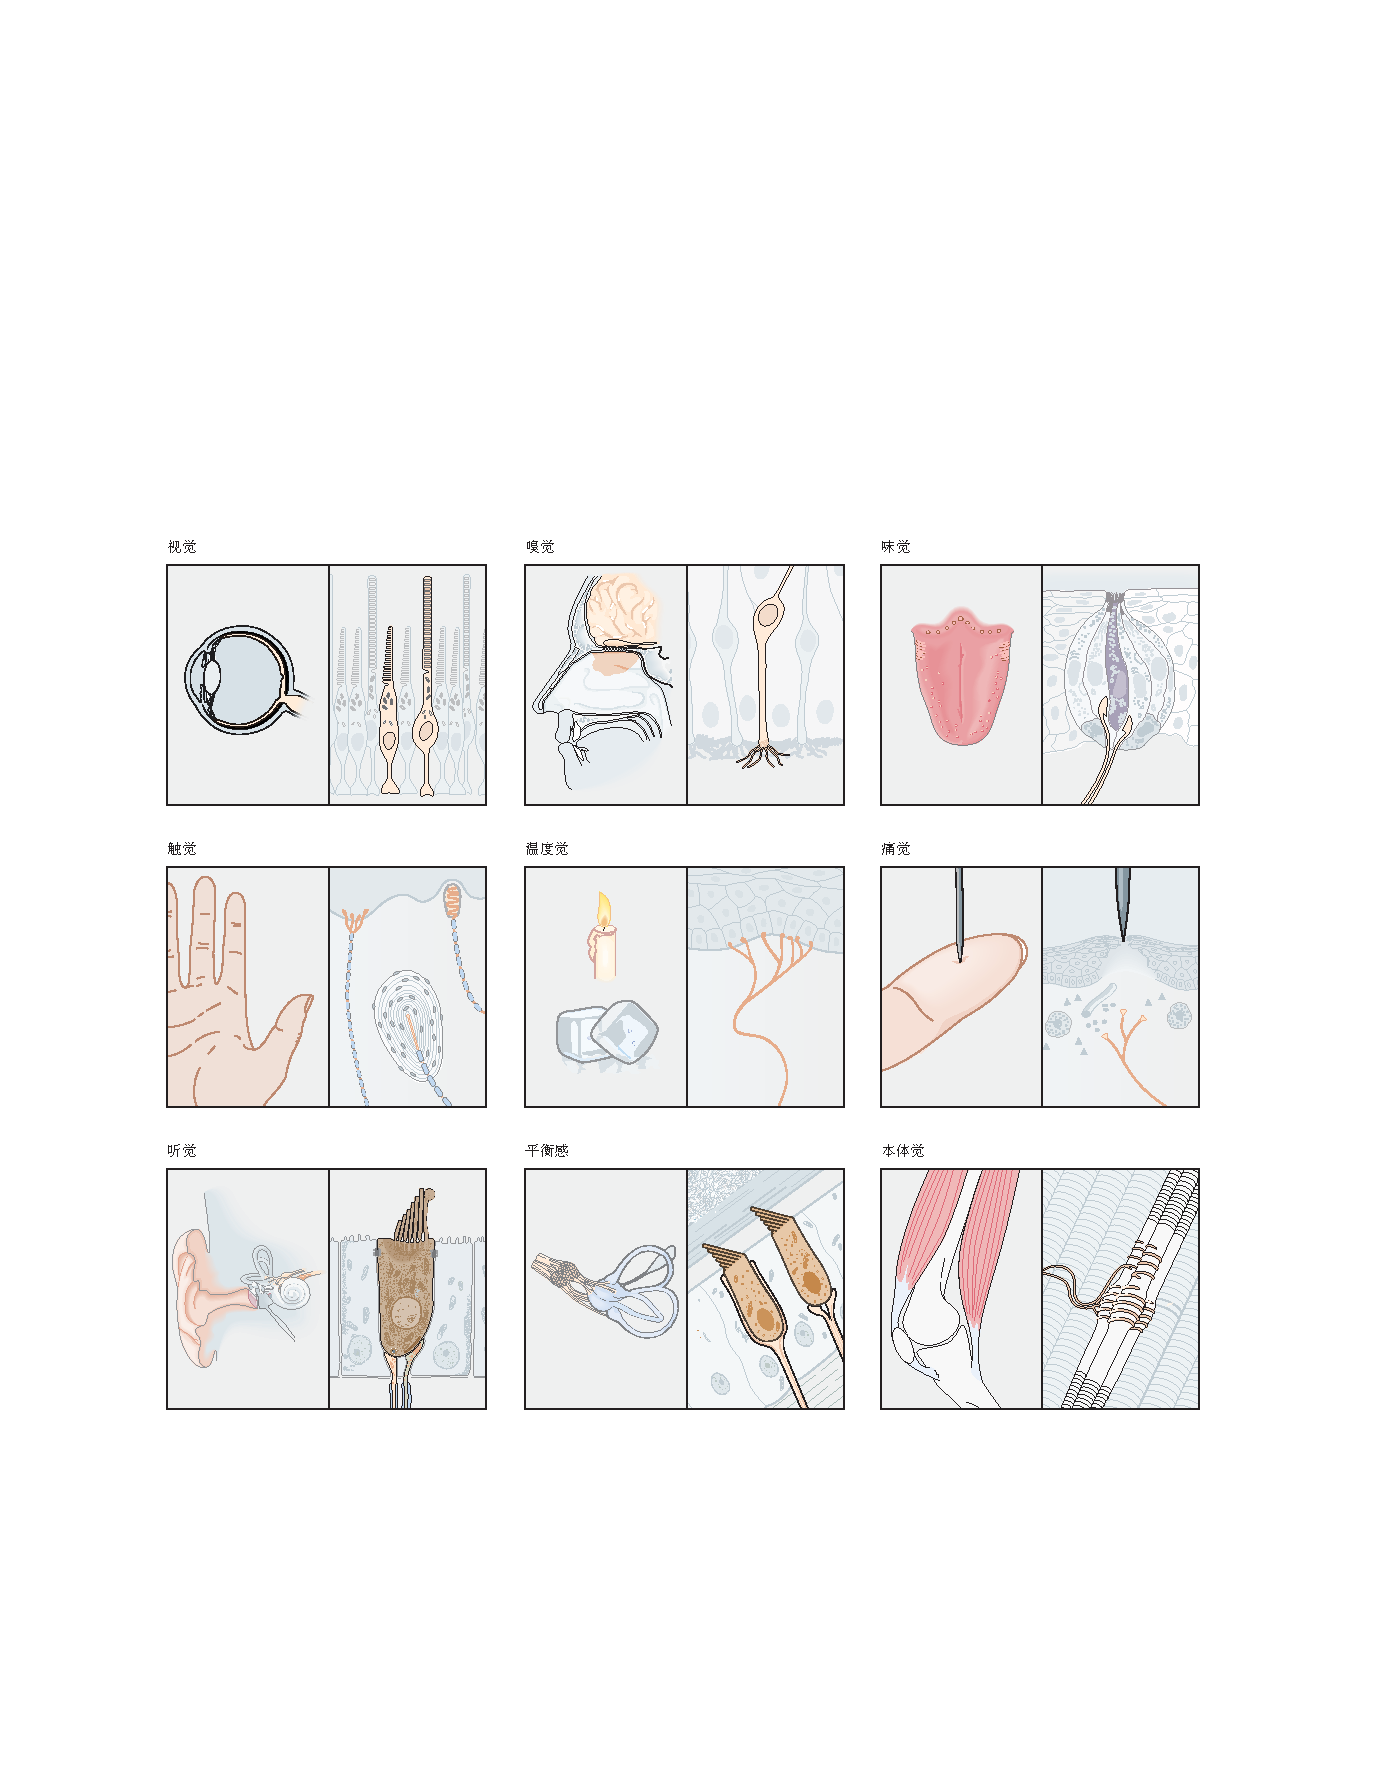
\includegraphics[width=1.0\linewidth]{chap17/fig_17_1}
	\caption{人类的主要感觉方式是由位于特定感觉器官中的不同类别的受体神经元介导的。 
		每一类受体细胞将一种类型的刺激能量转化为电信号,这些电信号被编码为动作电位序列(见图~\ref{fig:17_4})。 
		主要的感受器细胞包括光感受器(视觉)、化学感受器(嗅觉、味觉和疼痛)、热感受器和机械感受器(触觉、听觉、平衡和本体感受)。 
		经典的五种感觉——视觉、嗅觉、味觉、触觉和听觉——以及平衡感分别由眼睛、鼻子、嘴巴、皮肤和内耳中的感受器调节。 
		其他体感方式——热感、疼痛、内脏感觉和本体感觉——由分布在全身的受体介导。}
	\label{fig:17_1}
\end{figure}



感觉通路同时具有串行和并行组件,由具有数千或数百万个轴突的纤维束组成,这些轴突通过突触连接,传递和转换信息。 
受体对刺激的相对简单形式的神经编码通过大脑中复杂的机制进行调节,从而形成认知的基础。 
感觉通路也由大脑中的高级中枢控制,这些中枢通过将信息反馈回处理的早期阶段来修改和调节传入的感觉信号。 
因此,知觉不仅仅是“原始”物理感官信息的产物,也是认知和经验的产物。


科学家和哲学家都研究了我们体验到的感觉在多大程度上准确地反映了产生它们的刺激,以及它们是如何被我们对世界固有的主观和不精确的知识所改变的。 
在过去的几个世纪里,欧洲哲学家对感觉和知觉的兴趣与人性本身的问题有关。 
两种思想流派最终占据主导地位:以约翰·洛克、乔治·伯克利和大卫·休谟为代表的经验主义,
以及以勒内·笛卡尔、伊曼纽尔·康德和格奥尔格·威廉·弗里德里希·黑格尔为代表的唯心主义。


杰出的经验主义者洛克提出了这样的观点,即出生时的头脑是一块空白的石板,或白板,没有任何想法。 
他断言,知识只能通过感官体验获得——我们看到、听到、感觉到、尝到和闻到的东西。 
伯克利通过质疑在通过感官获得的经验和知识之外是否存在任何感官现实来扩展这一主题。 
他提出了一个著名的问题:如果没有人靠近,倒下的树会发出声音吗?


理想主义者认为,人类思维具有某些与生俱来的能力,包括逻辑推理本身。
康德将五种感官归类为人类理解的类别。
他认为,感知不是我们周围世界的直接记录,而是大脑的产物,因此取决于神经系统的结构。
康德将这些大脑特性称为先验知识。


因此,在康德看来,心灵并不是经验主义者设想的被动的感官印象接受者。 
相反,它已经进化为符合某些普遍条件,例如空间、时间和因果关系。 
这些条件与身体检测到的任何物理刺激无关。 
对于康德和其他唯心主义者来说,这意味着知识不仅基于感官刺激,还基于我们组织和解释感官体验的能力。 
他们说,如果感官体验本质上是主观的和个人的,那么它可能不受实证分析的影响。
随着对知觉的实证研究的成熟,两个学派都被证明是部分正确的。



\section{心理物理学将感觉与刺激的物理特性联系起来}

随着实验心理学作为一门科学学科的出现,对感觉和知觉的现代研究始于 19 世纪。 
第一批科学心理学家——恩斯特·韦伯、古斯塔夫·费希纳、赫尔曼·亥姆霍兹和威廉·冯特——将他们对心理过程的实验研究集中在感觉上,他们认为这是理解心灵的关键。 
他们的发现催生了心理物理学和感觉生理学领域。


心理物理学描述了刺激的物理特性与感官体验的属性之间的关系。 
感觉生理学检查刺激的神经后果——刺激如何被感觉受体转导并在大脑中进行处理。 
我们对感知的理解中一些最令人兴奋的进步来自于在人类和动物研究中合并这两种方法。 
例如,\textit{功能性磁共振成像}和\textit{正电子发射断层成像}已用于受控实验,以识别人脑中参与疼痛感知或识别特定类型物体或特定人物和地点的区域。


\subsection{心理物理学量化刺激特性的感知}

早期的心智科学研究并不关注对颜色或味道等复杂品质的感知,而是关注可以被隔离和精确测量的现象:刺激的大小、形状、幅度、速度和时间。 
\textit{韦伯}和\textit{费希纳}开发了简单的实验范式来研究人类如何以及在什么条件下能够区分两种不同振幅的刺激。 
他们以数学定律的形式量化了感觉的强度,使他们能够预测刺激强度与其可检测性之间的关系,包括区分不同刺激的能力。


1953 年,\textit{史蒂文斯}证明了刺激($ S $)强度($ I $)主观体验最好用幂函数来描述。 
史蒂文斯定律指出,
\begin{equation}
	I = K(S-S_0)^n,
\end{equation}
其中\textit{感觉阈值}($ S_0 $) 受试者可以检测到的最低刺激强度,$K$ 是一个常数。 
对于一些感觉,例如手上的压力感,刺激幅度与其感知强度之间的关系是线性的,即具有单位指数($ n = 1 $)的幂函数。


所有的感觉系统都有一个阈值,而阈值有两个基本功能。 
首先,通过询问一种感觉是否足够大以具有足够高的兴趣或相关概率,他们减少了对噪音的不必要反应。
其次,阈值引入的特定非线性有助于编码和处理,即使其他主要感觉反应与刺激成线性比例也是如此。
感觉阈值是一项功能,而不是错误。 
阈值通常是通过向受试者提供一系列随机幅度的刺激来统计确定的。
受试者报告检测到刺激的次数百分比绘制为刺激幅度的函数,形成称为心理测量函数的关系(图~\ref{fig:17_2})。 
按照惯例,阈值定义为在一半试验中检测到的刺激幅度。


\begin{figure}[htbp]
	\centering
	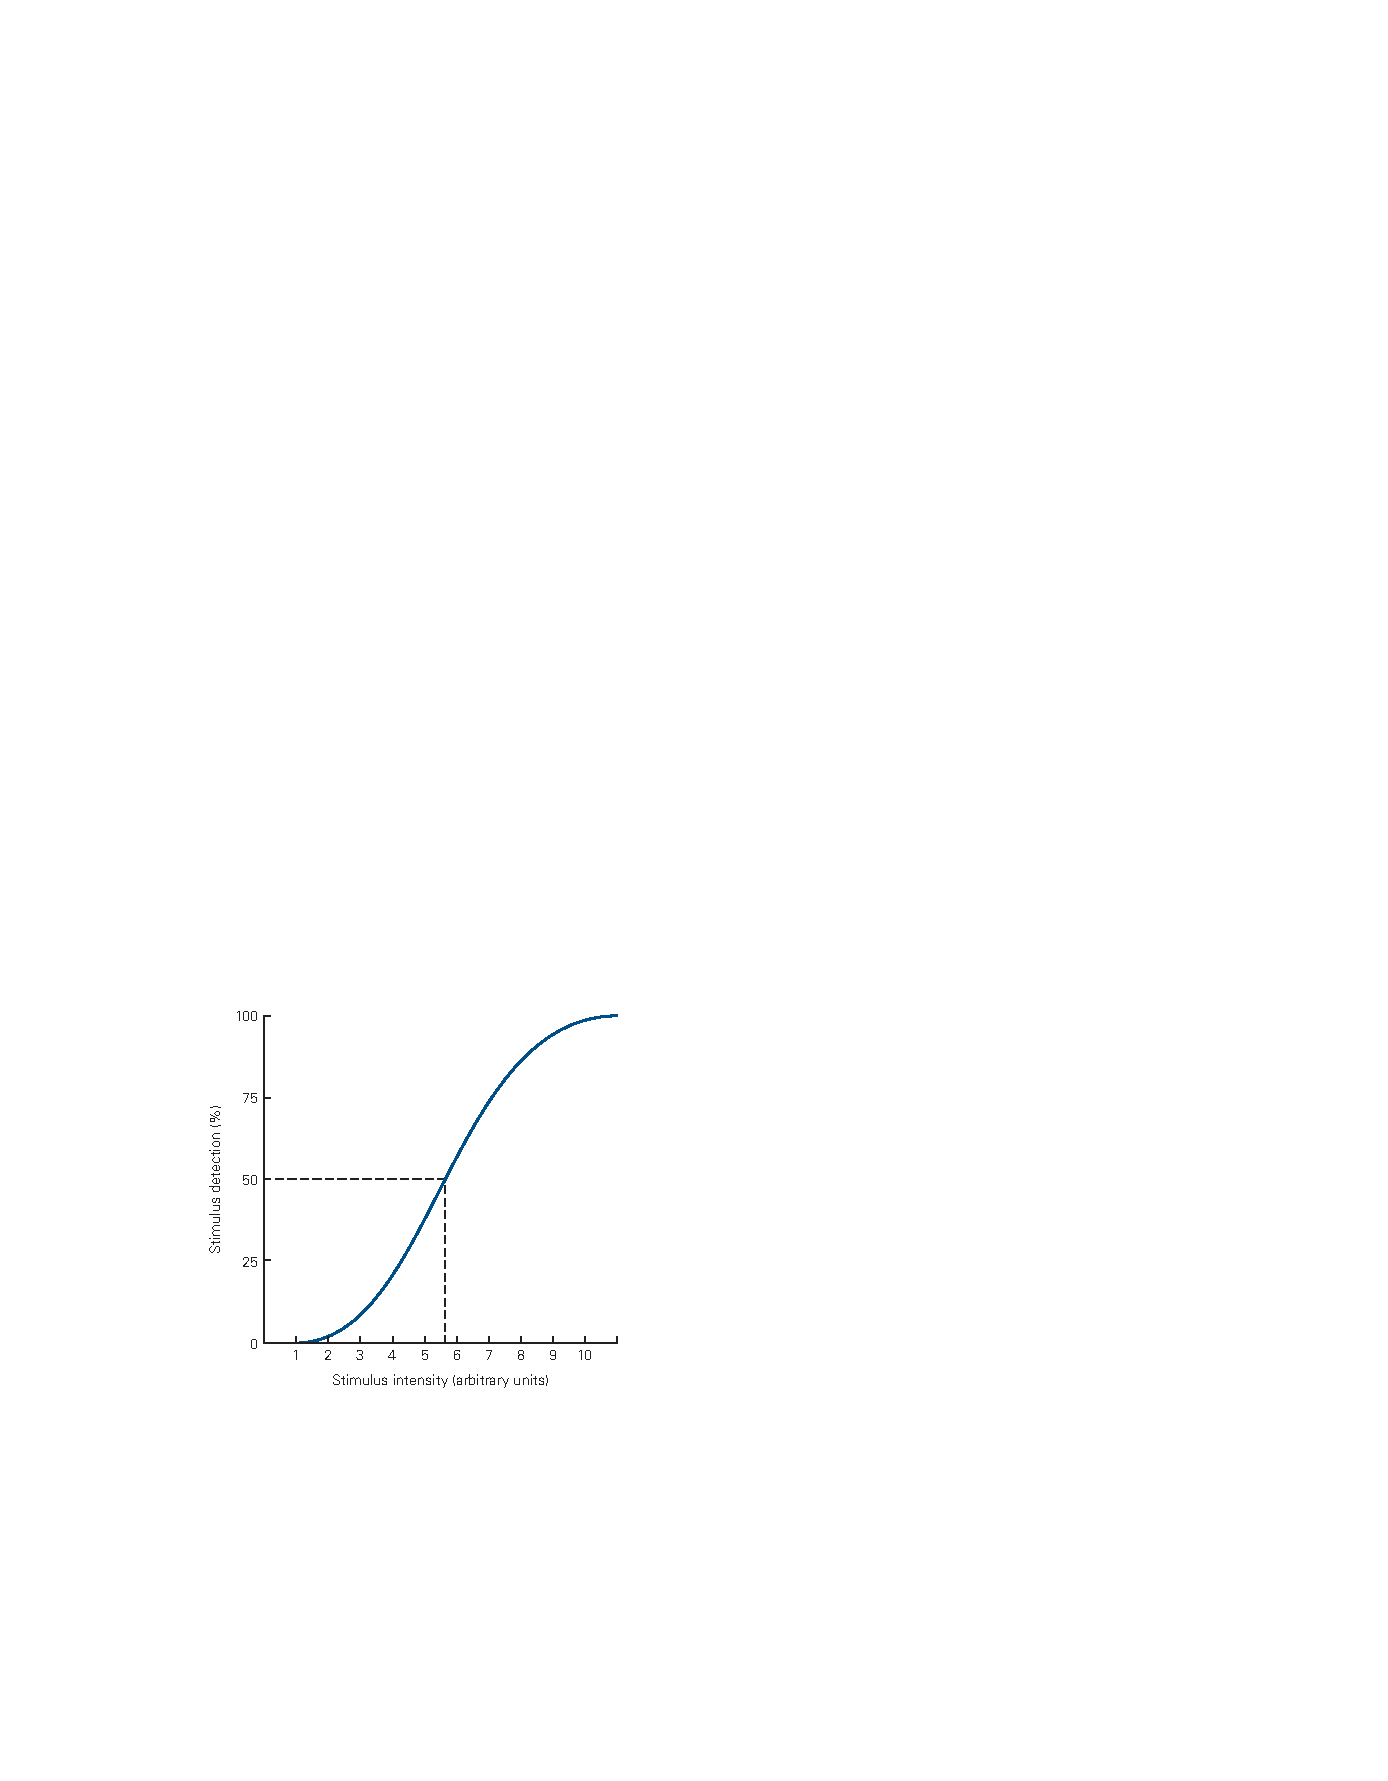
\includegraphics[width=0.5\linewidth]{chap17/fig_17_2}
	\caption{心理测量功能。 
		心理测量函数将人类观察者检测到的刺激百分比绘制为刺激幅度的函数。 
		阈值定义为在 50\% 的试验中检测到的刺激强度,在本例中约为 5.5(任意单位)。 
		心理测量函数还用于测量强度、频率或其他参数属性不同的刺激之间的\textit{最小可觉差}。}
	\label{fig:17_2}
\end{figure}


\begin{figure}[htbp]
	\centering
	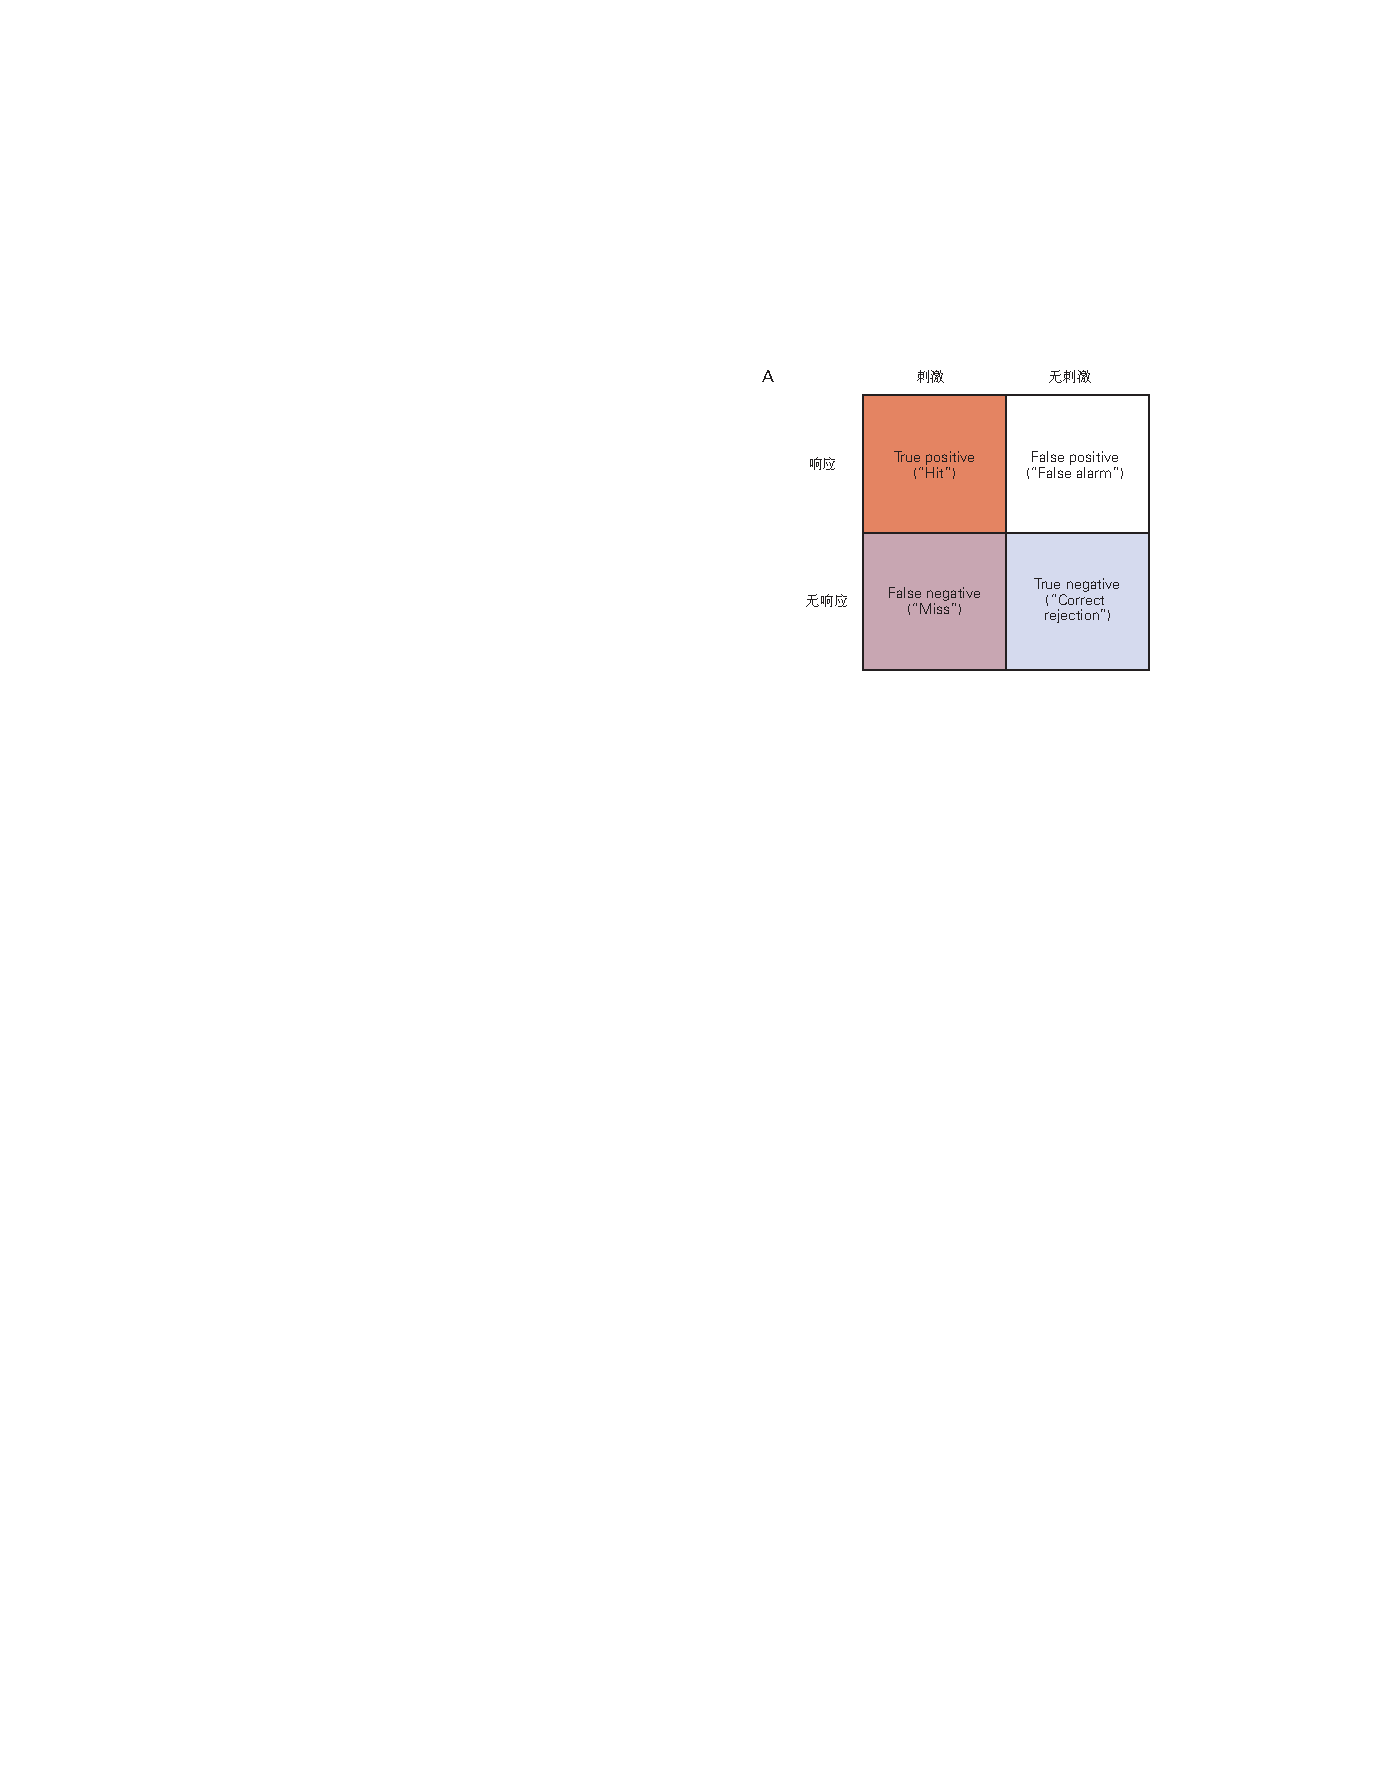
\includegraphics[width=0.5\linewidth]{chap17/fig_17_3_a}
	\caption{在是-否刺激检测任务期间收集的数据的刺激-响应矩阵(“那里有特定的刺激吗?”)。
		每次试验都会更新四个总数中的一个。
		例如,正确检测刺激会更新真阳性(命中)的计数,但在没有刺激的情况下错误的阳性反应将被视为假阳性。
		从这样的表中,可以计算出敏感度和假阳性率等重要指标。}
	\label{fig:17_3_a}
\end{figure}


\begin{figure}[htbp]
	\centering
	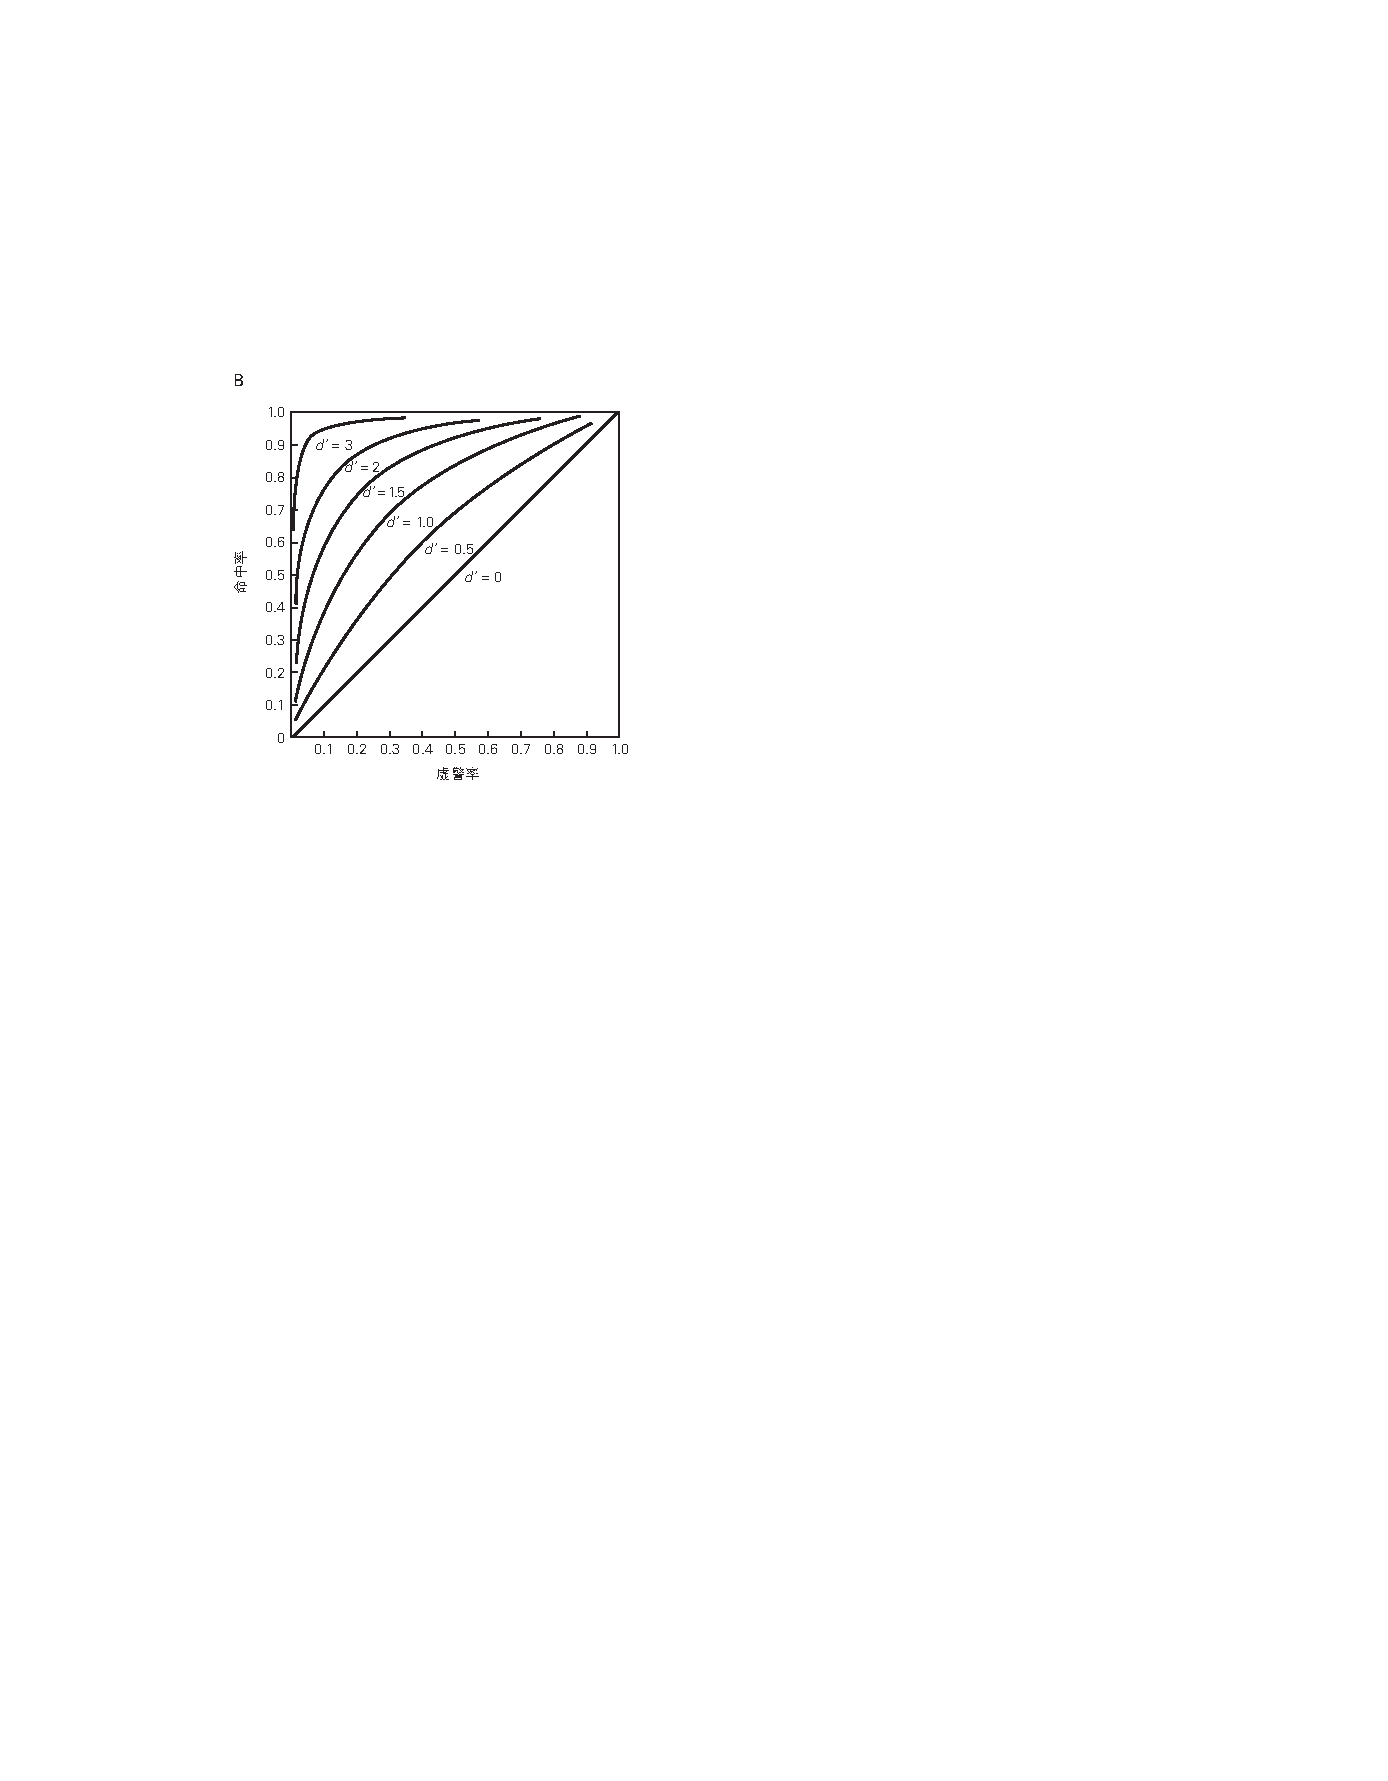
\includegraphics[width=0.5\linewidth]{chap17/fig_17_3_b}
	\caption{\textit{受试者工作特征}图显示试验集的结果,每个试验都收集在如图~\ref{fig:17_3_a}A~所示的矩阵中。
		垂直轴绘制了命中率或概率作为水平轴上误报率或概率的函数。
		标记垂直轴 TPR(真阳性率)或灵敏度,以及标记水平轴 FPR(假阳性率)或(1 - 特异性)也很常见。
		随机提供是或否响应的一组试验(可辨别性 [d'] = 0)绘制为从原点到右上角的直线。
		这种\textit{受试者工作特征}的\textit{曲线下面积}将为 0.5。
		一组完美的试验,其中观察者准确地检测到每个刺激的存在并且不会被任何没有刺激的试验所愚弄(d'> 3),将沿着左轴急剧上升,并且\textit{曲线下面积}将为 1.0。
		\textit{曲线下面积}值越来越多地被引用为单个数字的置信度度量。
		所示的(理论)曲线证明了 d ' 的较高值如何导致较大的\textit{曲线下面积}\cite{swets1973relative}。}
	\label{fig:17_3_b}
\end{figure}


感觉阈值的测量是诊断个体模式中感觉功能的有用技术。 
升高的阈值可能表示感觉受体异常(例如由于衰老或暴露于非常大的噪音引起的内耳毛细胞丢失)、神经传导特性缺陷(如多发性硬化症)或感觉处理区域的病变的大脑。
与测量刺激检测的条件相关的情绪或心理因素也可能改变感觉阈值。
阈值也可以通过极限法来确定,其中受试者报告逐渐减少的刺激不再可检测到或增加的刺激变得可检测到的强度。
该技术在听力学中广泛用于测量听力阈值。


受试者还可以使用杠杆、按钮或其他允许准确测量决策时间的设备,在感官检测或辨别任务中提供非语言反应。 
可以使用此类设备训练实验动物对受控的感官刺激做出反应,从而使神经科学家能够通过在同一实验中结合电生理学和行为学研究来研究潜在的神经机制。
方框~\ref{box:17_1}~中总结了量化对刺激的反应的方法。


\begin{proposition}[信号检测理论:量化检测和鉴别] \label{box:17_1}
	
	\quad \quad 我们的感觉系统的两个主要功能是告诉我们是否有什么东西以及它是什么。
	为了测试我们的能力以及我们的感觉系统回答这些问题的能力,已经开发了实验方案,工具和方法来量化感觉系统对刺激的反应。
	这些理论包括决策理论和信号检测理论。
	每种方法都使用统计方法来量化受试者反应的可变性。
	
	\quad \quad 例如,在“有什么东西吗?”任务中,受试者或实验动物可以正确地检测到特定的刺激(“命中”或“真阳性”),在没有该刺激的情况下反应不正确(“假阳性”或“假警报”),对真正刺激没有反应(“错过”),或者在没有刺激的情况下正确拒绝回应(“真正的负面”或“正确的拒绝”)。
	通过反复演示,这些选择可以列在四细胞刺激-反应矩阵中(图~\ref{fig:17_3_a}A)。
	
	\quad \quad 这量化了敏感性,定义为真实阳性的数量除以所呈现的刺激的数量,以及特异性,定义为真实阴性的数量除以没有刺激的呈现的数量。
	
	\quad \quad 1927年,L.L.Thurstone提出,刺激引起的感觉变化可以表示为正态或高斯概率函数,将两个刺激幅度之间的物理距离等于推断强度的心理尺度值,称为辨别指数或d'。
	
	\quad \quad 1954年,心理学家威尔逊·坦纳(WilsonTanner)和约翰·斯维茨(JohnSwets)首次将决策理论方法应用于心理物理学研究。
	他们开发了一系列刺激检测实验方案,可以准确计算d'以及定量分析人类和动物受试者感觉的技术。
	这样的研究不仅可以像前面的例子那样测量“有什么东西吗?”还可以测量刺激的物理特性(如强度,大小或时间频率)的比较判断,从而测量“它是什么?”的两种替代强迫选择类似物。
	
	\quad \quad 当受试者被要求报告第二个刺激是否比第一个刺激更强或更弱,更高或更低,更大或更小,或相同或不同时,每个试验中的反应可以再次列在四细胞刺激-反应矩阵中,类似于图17-3A中的矩阵,但术语“刺激”或“无刺激”被两个不同的刺激所取代。
	
	\quad \quad 这些研究中的辨别力(d')是通过\textit{受试者工作特征}分析来测量的,该分析比较了由某些性质不同的刺激对引起的神经放电率或选择概率。
	假设两种刺激中的一种会引起比另一种更高的反应。
	当决策标准设置为不同的射击水平或选择率时,神经或心理物理数据的\textit{受试者工作特征}图绘制了正确判断(命中)和错误判断(假阳性)的试验比例(图~\ref{fig:17_3_b}B)。
	\textit{受试者工作特征}曲线下的面积为每个刺激对提供了d'的准确估计。
	
	\quad \quad William Newsome,Michael Shadlen和J.Anthony Movshon已经将信号检测方法应用于研究神经对视觉刺激的反应,这些视觉刺激在方向,空间频率或运动连贯性方面有所不同,以便将神经放电率的变化与感觉处理相关联。
	神经测量功能将神经辨别力绘制为刺激差异的函数,与在测试相同刺激的强制选择范例中获得的心理测量功能密切相关,从而为观察到的行为反应提供了生理基础。
	
	\quad \quad 这些工具中的许多部分是为了研究感觉系统而开发的,已经被广泛应用于神经科学以外的领域。
	\textit{受试者工作特征}曲线,敏感性和特异性对于量化疾病的诊断和治疗至关重要。
	\textit{受试者工作特征}的\textit{曲线下面积}今天比d'使用得多。
	接近1的\textit{曲线下面积}值表征高灵敏度和高特异性。
	对于许多真阳性结果很少的实验或临床研究,假阳性率(1-特异性,或假阳性数除以无刺激的呈现数)比经典$ p $值更有意义。
	
\end{proposition}



\section{刺激在神经系统中由神经元的放电模式表示}
心理物理学方法为分析刺激引起的感觉提供了客观的技术。 
这些定量测量已与神经生理学技术相结合,以研究将感觉神经信号转化为知觉的神经机制。 
感觉神经科学的目标是追踪从受体到大脑认知中心的感觉信息流,了解连续突触发生的处理机制,并破译它如何塑造我们对外部世界的内部表征。 
感觉信息的神经编码在处理的早期阶段比在大脑的后期阶段更容易理解。


这种解决神经编码问题的方法在 1960 年代由\textit{弗农·芒卡斯尔}率先提出,他表明来自外周和中枢感觉神经元的尖峰序列的单细胞记录提供了对物理刺激诱发的神经活动的统计描述。
然后他研究了神经反应的哪些定量方面可能对应于感官任务的心理物理测量,同样重要的是,哪些不对应。


信息的神经编码研究是理解大脑如何工作的基础。
神经代码描述了特定神经群体中的活动与其对感知或行动的功能性后果之间的关系。 
感觉系统是神经编码研究的理想选择,因为这些系统的刺激输入的物理特性和神经或行为输出都可以在受控环境中精确定义和量化。


通过记录感觉处理各个阶段的神经元活动,神经科学家试图破译各种感觉方式用来表示信息的机制,以及将这些信号传递给由动作电位序列编码的大脑所需的转换。 
对神经网络沿着通往大脑皮层和在大脑皮层内的通路进行的信号转换进行了额外的分析。 
神经科学家还可以通过电脉冲、化学神经递质和调节剂的直接刺激来改变感觉回路中的活动,或者可以使用基因编码的光激活离子通道(光遗传学)来使感觉神经元去极化或超极化。 
神经元如何对感觉刺激进行编码可能会导致深入了解构成认知基础的编码原则。


人们常说,大脑的力量在于数以百万计的神经元并行处理信息。 
然而,这种表述并没有抓住大脑与身体所有其他器官之间的本质区别。 
在肾脏或肌肉中,大多数细胞做着类似的事情; 
如果我们了解典型的肌肉细胞,我们基本上就会了解整个肌肉是如何工作的。 
在大脑中,数百万个细胞各自做着不同的事情。 
要了解大脑,我们需要了解它的任务是如何在神经元网络中组织的。



\subsection{感觉受体对特定类别的刺激能量有反应}

感觉系统之间的功能差异源于两个特征:驱动它们的不同刺激能量和构成每个系统的离散通路。 
每个神经元执行特定的任务,它产生的一系列动作电位对该回路中的所有突触后神经元具有特定的功能意义。 
这一基本思想在 19 世纪由查尔斯·贝尔和约翰内斯·米勒提出的特异性理论中得到表达,至今仍是感觉神经科学的基石之一。


在分析感官体验时,重要的是要认识到我们的意识感觉与刺激的物理特性在性质上是不同的,因为正如康德和唯心主义者所预测的那样,神经系统仅提取每个刺激的某些特征而忽略其他特征。 
然后,它会在大脑的内在结构和先前经验的限制下解释这些信息。 
因此,我们接收到不同频率的电磁波,但我们将它们视为颜色。 
我们从以不同频率振动的物体接收压力波,但我们听到声音、文字和音乐。 
我们遇到漂浮在空气或水中的化合物,但我们将它们体验为气味和味道。 
颜色、色调、气味和味道是大脑根据感官经验构建的精神创造。 
它们本身并不存在于大脑之外,而是与刺激的特定物理特性相关联。


丰富的感官体验始于数百万个高度特异性的感觉受体。 
感觉受体存在于称为感觉器官的特殊上皮结构中,主要是眼睛、耳朵、鼻子、舌头和皮肤。 
每个受体在感觉器官的特定位置对特定类型的能量作出反应,有时仅对具有特定时间或空间模式的能量作出反应。 
受体将刺激能量转化为电能; 
因此,所有感觉系统都使用共同的信号机制。 
受体产生的电信号的幅度和持续时间,称为受体电位,与受体刺激的强度和时间进程有关。
特定刺激能量转化为电信号的过程称为刺激转导。


感觉受体在形态上专门用于转导特定形式的能量,并且每个受体在感觉器官内都有一个专门的解剖区域,刺激转导发生在该区域(图~\ref{fig:17_4})。 
大多数受体对单一类型的刺激能量具有最佳选择性,这种特性称为受体特异性。
例如,我们看到特定的颜色是因为我们有对特定波长范围的光子选择性敏感的受体,我们闻到特定的气味是因为我们有结合特定气味分子的受体。


\begin{figure}[htbp]
	\centering
	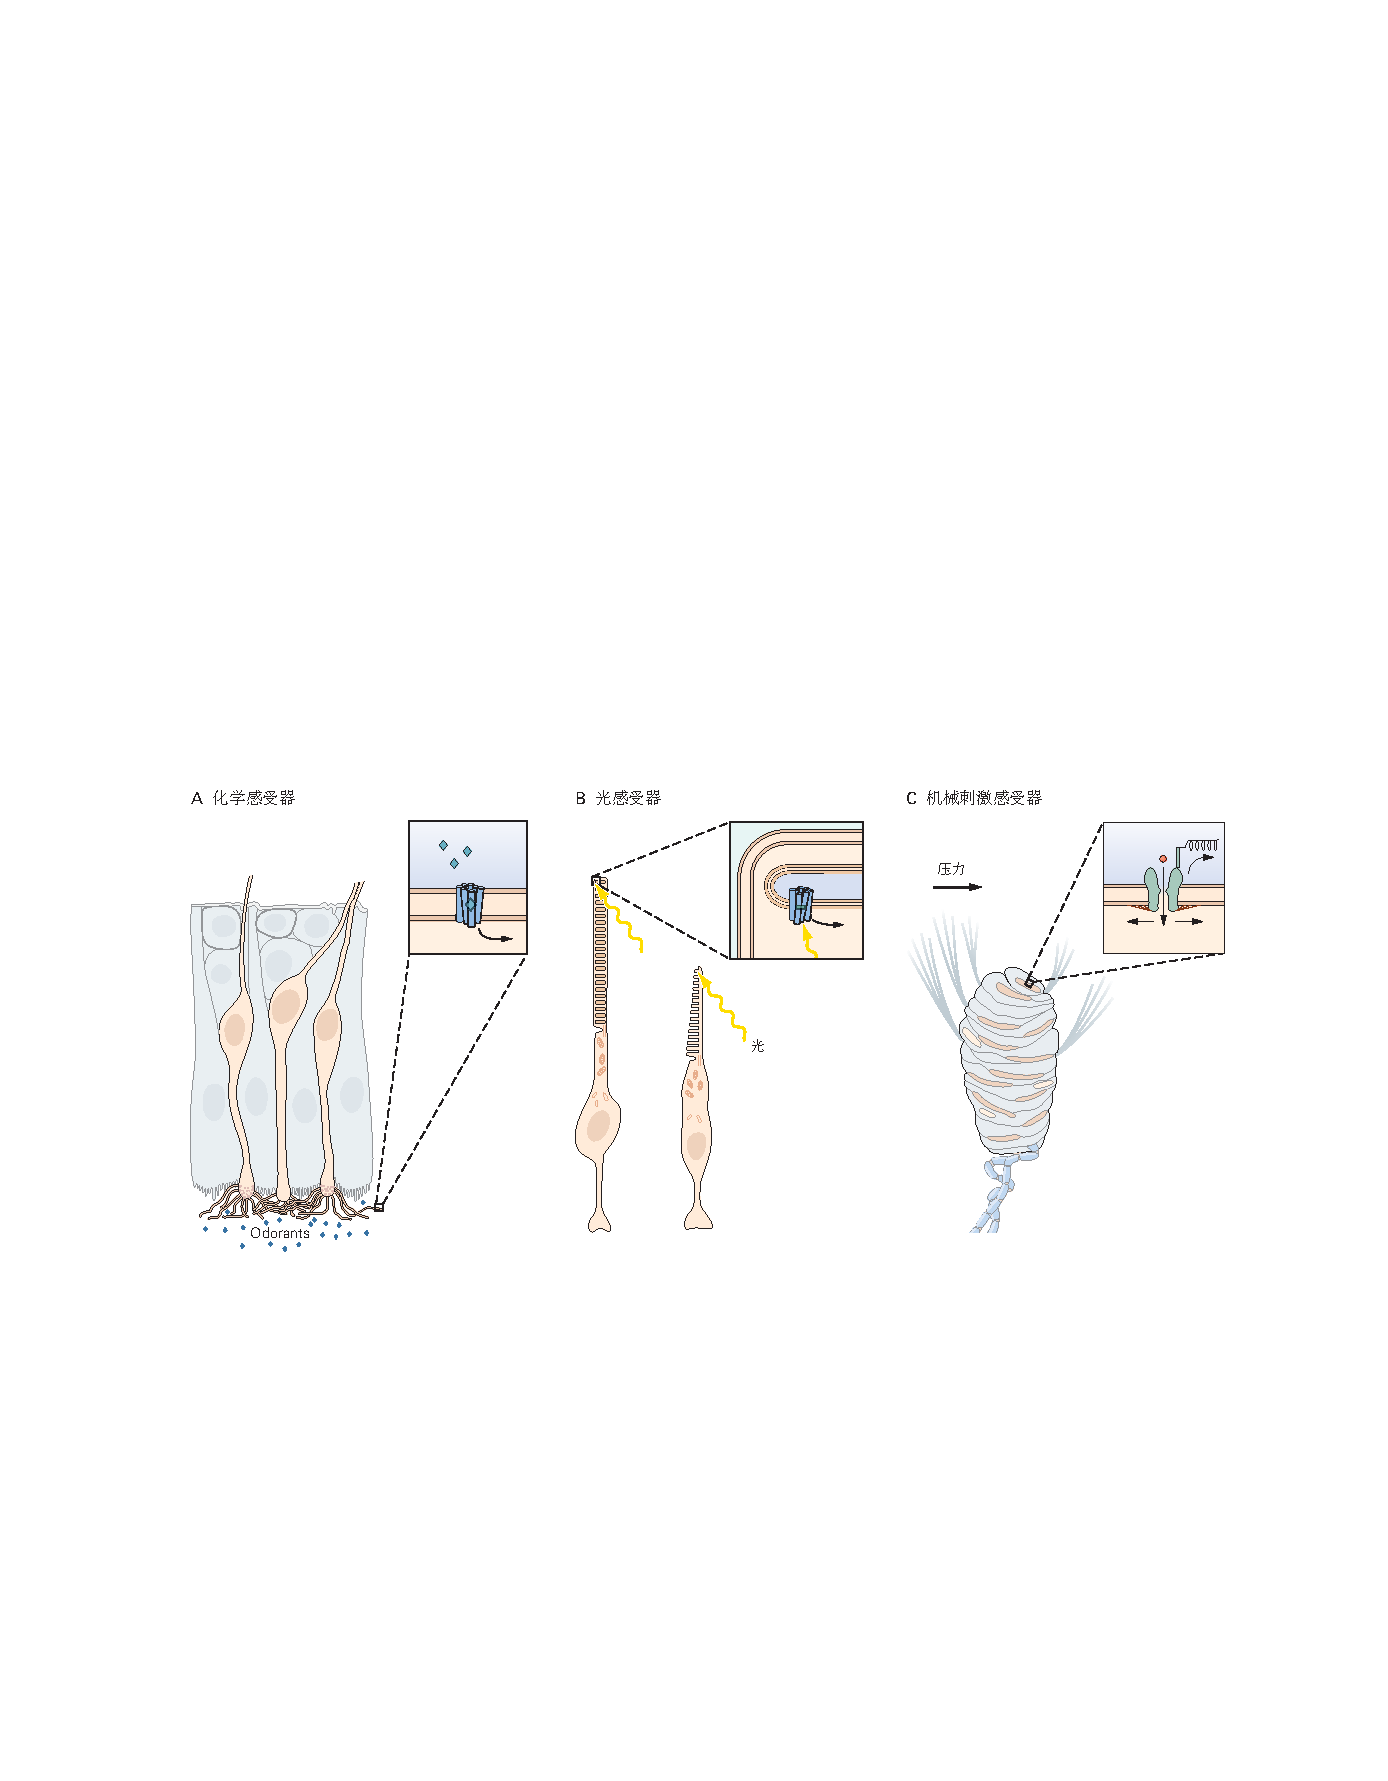
\includegraphics[width=1.0\linewidth]{chap17/fig_17_4}
	\caption{感觉受体专门将特定类型的刺激能量转换为电信号。 
		感觉受体根据激发它们的刺激能量类别分为化学感受器、光感受器或机械感受器。
		它们将这种能量转化为电信号,沿着服务于一种感觉方式的通路传输。
		每个面板中的插图说明了被刺激激活的离子通道的位置。
		\textbf{A.} 嗅毛细胞对空气中的化学分子作出反应。
		粘膜表面的嗅觉纤毛结合特定的气味分子,并通过第二信使系统使感觉神经去极化。
		激活率表示吸入空气中气味剂的浓度。
		\textbf{B.} 视网膜中的视杆细胞和视锥细胞对光有反应。
		两个受体的外段都含有感光色素视紫红质,当它吸收特定波长的光时会改变构型。
		光对发色团的刺激降低了细胞质中环鸟苷 3',5'-单磷酸 (cGMP) 的浓度,关闭阳离子通道,从而使光感受器超极化\cite{shepherd1988neurobiology}。
		\textbf{C.} Meissner 的小体对机械压力有反应。 
		感觉神经末梢(粉红色)周围充满液体的胶囊(淡蓝色)通过胶原纤维连接到指纹脊。
		皮肤上的压力或运动会打开神经纤维末梢中的拉伸敏感离子通道,从而使它们去极化\cite{albe1973morphology}。}
	\label{fig:17_4}
\end{figure}


在所有的感觉系统中,每个受体都会编码施加到其感受野的能量类型、局部刺激强度以及它如何随时间变化。
例如,视网膜中的光感受器对从视野中特定位置照射到视网膜的光的色调、亮度和持续时间进行编码。
耳蜗中的毛细胞感受器对击中耳朵的声压波的音调频率、响度和持续时间进行编码。
因此,物体、声音或场景的神经表征由单个受体的马赛克组成,这些受体共同发出其大小、轮廓、纹理、时间频率、颜色和温度的信号。


感觉器官中受体的排列允许每个感觉系统内的功能进一步专门化。 
哺乳动物的感觉受体分为机械感受器、化学感受器、光感受器或温度感受器(表~\ref{tab:17_1})。
机械感受器和化学感受器分布最广,形式和功能也最多样。


\begin{table}[htbp]
	\centering
	\caption{感觉受体的分类}
	\begin{tabular}{lllll}
		\toprule
		感觉系统 & 模态 & 刺激 & 受体类型 & 受体细胞 \\
		\midrule
		视觉 & 视觉 & 光(光子)   & 光感受器 & 视杆细胞核视锥细胞\\
		听觉 & 听觉 & 声音   & 机械刺激感受器 & 耳蜗中的毛细胞 \\
		前庭觉 & 头动 & 重力、加速度和头动   & 机械刺激感受器 & 前庭迷路中的毛细胞 \\
		躯体感觉 &  &   &  & \makecell{具有以下受体的颅骨 \\ 和背根神经节细胞:} \\
		 & 触觉 & 皮肤变形和运动   & 机械刺激感受器 & 皮肤 \\
		 & 本体感觉 & 肌肉长度、肌肉力量和关节角度   & 机械刺激感受器 & \makecell{肌梭、高尔基肌腱 \\ 器官和关节囊}  \\
		 & 痛觉 & 有害刺激(热、机械和化学刺激)  & \makecell{机械刺激感受器、 \\ 温度感受器和化学感受器}  & \makecell{除中枢神经系统外 \\ 的所有组织}  \\
		 & 痒觉 & 组胺,pruritogens  & 化学感受器 & 皮肤 \\
		 & 内脏觉 & 范围广(热、机械和化学刺激)  & \makecell{机械刺激感受器、 \\ 温度感受器和化学感受器} & \makecell{心血管、胃肠道、 \\ 膀胱和肺}  \\
		味觉 & 味道 & 化学剂   & 化学感受器 & \makecell{味蕾、口腔内热 \\ 和化学感受器}  \\
		嗅觉 & 气味 & 气味剂   & 化学感受器 & 嗅感觉神经元 \\
		\bottomrule
	\end{tabular}%
	\label{tab:17_1}%
\end{table}%


感知皮肤变形、运动、拉伸和振动的四种不同类型的机械感受器负责人手和其他地方的触觉(第~\ref{chap:chap18}~和~\ref{chap:chap19}~章)。 
肌肉包含三种机械感受器,它们会发出肌肉长度、速度和力的信号,而关节囊中的其他机械感受器会发出关节角度信号(第~\ref{chap:chap31}~章)。 
听力基于两种机械感受器,内毛细胞和外毛细胞,它们转换内耳基底膜的运动(第~\ref{chap:chap26}~章)。 
前庭迷路中的其他毛细胞感知内耳液体的运动和加速,以发出头部运动和方向的信号(第~\ref{chap:chap27}~章)。 
内脏机械感受器检测肠和膀胱等内脏器官的扩张。 
当细胞膨胀时,大脑中感知水合状态的渗透压感受器就会被激活。 
某些机械感受器报告有可能损坏组织的极端变形; 
它们的信号到达大脑中的疼痛中心(第~\ref{chap:chap20}~章)。


化学感受器负责嗅觉、味觉、瘙痒、疼痛和许多内脏感觉。 
疼痛的很大一部分是由于化学感受器检测到因组织损伤而溢出到细胞外液中的分子和作为炎症反应一部分的分子。 
皮肤中的几种温度感受器感知皮肤变暖和变冷。 
另一种温度感受器监测下丘脑的血液温度,主要负责我们是否感到温暖或寒冷。


视觉由视网膜中的五种光感受器介导。 
这些受体的光敏感性定义了可见光谱。 
视杆细胞和视锥细胞中的感光色素检测波长范围为 390 至 670 纳米的电磁能(图~\ref{fig:17_5}A),这是到达地球并通知我们视觉世界的日光和月光的主要波长。 
与鸟类或爬行动物等其他一些物种不同,人类无法检测到紫外线或红外线辐射,因为我们缺乏检测适当的短波长或长波长的受体。 
同样,我们不会感知无线电波和微波能带,因为我们还没有进化出这些波长的受体。


\begin{figure}[htbp]
	\centering
	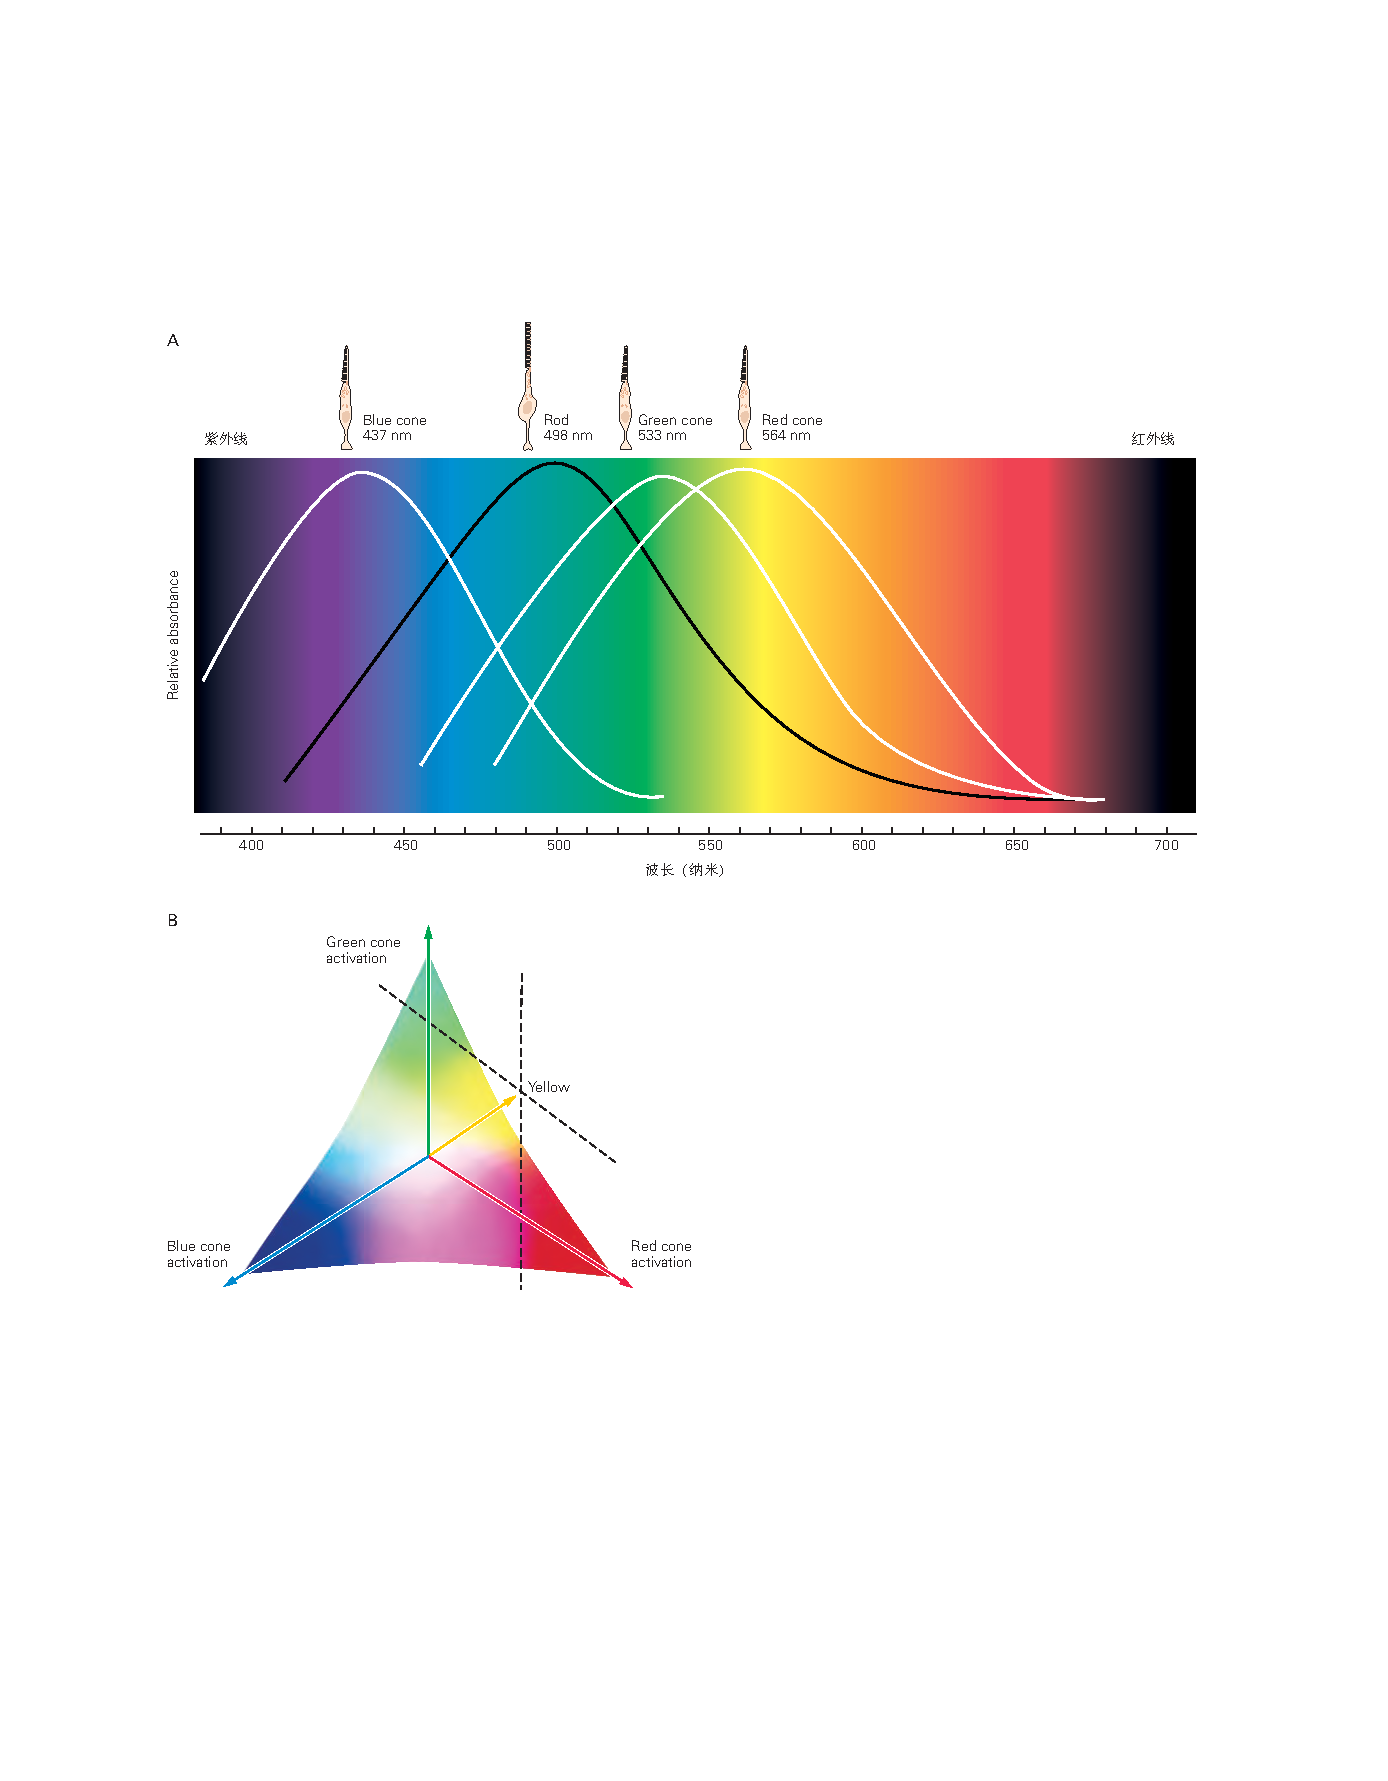
\includegraphics[width=1.0\linewidth]{chap17/fig_17_5}
	\caption{人类对颜色的感知来自于视网膜中三种不同类别的光感受器的同时激活。 
		\textbf{A.} 可见光谱的波长范围为 390 至 670 纳米。 
		单个感光器对宽范围的波长敏感,但每个感光器对特定光谱带中的光最敏感。 
		因此,视锥细胞被分类为红色、绿色或蓝色型光感受器。 
		三种锥体类型中每一种的相对激活的变化都解释了对特定颜色的感知~\cite{dowling1987retina}。
		\textbf{B.} 视网膜中颜色和亮度的神经编码可以描绘为三维向量,其中每种视锥细胞类型的激活强度沿三个轴之一绘制。 
		向量空间中的每个点代表三种锥体类型的独特激活模式。
		向量中的方向表示每种锥体类型的相对活动和看到的颜色。
		在此处显示的示例中,红色视锥细胞的强烈激活以及绿色视锥细胞的适度刺激和蓝色视锥细胞的弱激活产生了黄色的感知。
		从原点到该点的矢量长度表示视网膜该区域的光强度或亮度。}
	\label{fig:17_5}
\end{figure}



\subsection{每个感觉器官都有多个感觉受体亚类}

每个主要的感觉系统都有几个子模态。 
例如,味道可以是甜的、酸的、咸的、咸的或苦的; 
视觉对象具有颜色、形状和图案的特性; 
触觉包括温度、质地和硬度的特性。 
一些子模态由受体的离散子类介导,这些子类对该模态的刺激能量的有限范围作出反应; 
其他的是通过组合来自不同受体类型的信息而得出的。


受体充当窄范围或窄能量带宽的过滤器。 
例如,单个感光器并不对所有波长的光敏感,而只对光谱的一小部分敏感。 
我们说受体被调谐到最佳或最佳刺激,即以低能量激活受体并引起最强神经反应的首选刺激。 
因此,我们可以根据生理实验绘制每个受体的调谐曲线(参见图~\ref{fig:17_5}A~中光感受器的光吸收曲线)。 
调谐曲线显示受体的灵敏度范围,包括其首选刺激。
例如,视网膜中的蓝色视锥细胞对 430 至 440 纳米的光最敏感,绿色视锥细胞对 530 至 540 纳米的光反应最好,而红色视锥细胞对 560 至 570 纳米的光反应最强烈。 
三个视锥细胞对其他波长光的响应较弱,因为入射波长不同于这些最佳范围(第~\ref{chap:chap22}~章)。


因此,每个视杆细胞和视锥细胞都会对多种颜色做出反应。 
光感受器的分级灵敏度通过诱发受体电位的振幅对特定波长进行编码。 
然而,这个振幅还取决于光的强度或亮度,因此绿色圆锥体对明亮的橙色或较暗的绿色光的反应相似。 
这些怎么区分? 
较强的刺激比较弱的刺激激活更多的光感受器,由此产生的多个受体的群体代码,与不同波长偏好的受体相结合,可以区分强度和色调。 
这种神经集合使单个视觉神经元能够在同一通路中复用颜色和亮度信号。


此外,由于感光器的调谐曲线大致围绕最佳频率对称,因此较大或较小值的波长可能会引起类似的响应。 
例如,红色视锥细胞对 520 和 600 纳米的光有类似的反应。 
大脑如何解释这些信号? 
答案再次在于多个受体,在这种情况下是绿色和蓝色视锥细胞。 
绿色视锥细胞对 520 纳米的光反应非常强烈,因为它接近它们的首选波长,但对 600 纳米的光反应微弱。 
蓝色视锥细胞对 600 纳米的光没有反应,并且在 520 纳米时几乎没有被激活。 
因此,520 纳米的光被视为绿色,而 600 纳米的光被视为橙色。 
因此,通过光感受器的不同组合,我们能够感知到一系列颜色。


同样,我们在进食时感知到的复杂味道是对天然配体具有不同亲和力的化学感受器组合的结果。 
大量不同的嗅觉和味觉受体的广泛调谐曲线提供了许多组合的可能性。


亚模态的存在表明了感官编码的一个重要原则,即刺激能量的范围——例如光的波长——被解构为更小、更简单的成分,其强度随着时间的推移由专门的受体监测,这些受体并行传输信息 大脑。
大脑最终整合了这些不同的刺激成分,以传达感官事件的整体表现。 
当我们检查中枢神经系统中感觉事件的表征时,整体假说更为重要。 
尽管大多数关于感觉处理的研究都检查了单个神经元如何响应随时间变化的刺激,但当前的挑战是破译感觉信息如何分布在同时响应同一事件的神经元群体中。


\subsection{受体群编码将感觉信息传递给大脑}

由适当刺激产生的受体电位会产生感觉受体神经元的局部去极化或超极化,其振幅与刺激强度成正比。 
然而,感觉器官距离中枢神经系统足够远,受体电位的被动传播不足以在那里传输信号。 
为了将感觉信息传递给大脑,必须进行神经编码的第二步。 
刺激产生的受体电位必须转化为可沿轴突传播的动作电位序列。 
受体电位中刺激幅度的模拟信号被转换为数字脉冲代码,其中动作电位的频率与刺激强度成正比(图~\ref{fig:17_6}A)。 
这是脉冲序列编码。


\begin{figure}[htbp]
	\centering
	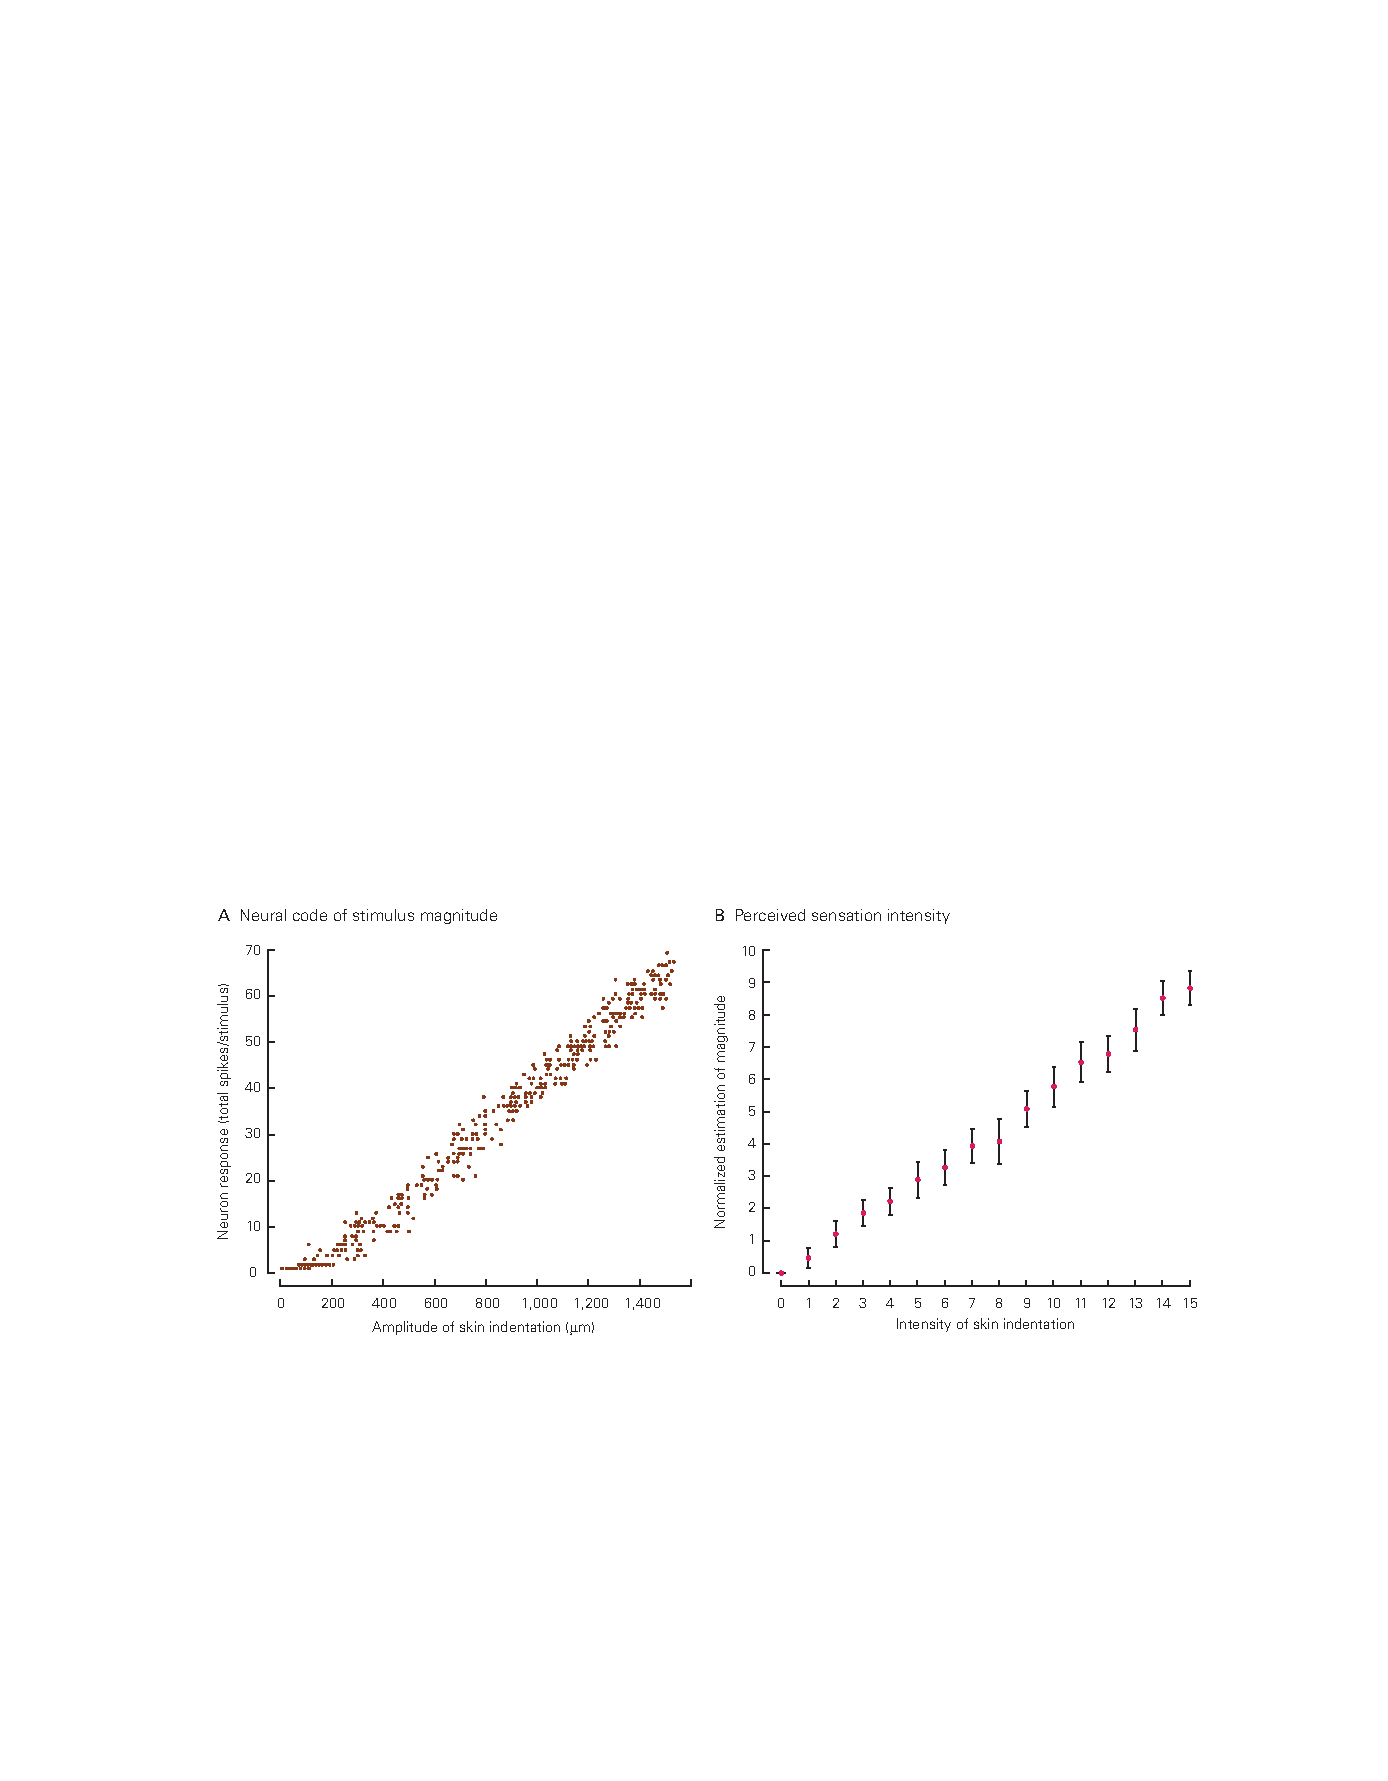
\includegraphics[width=1.0\linewidth]{chap17/fig_17_6}
	\caption{感觉神经元的放电率编码刺激强度。 
		这两个图表明刺激强度的神经编码忠实地从外周受体传输到介导意识感觉的皮层中心\cite{mountcastle1966neural}。
		\textbf{A.} 从手中的触觉感受器记录的每秒动作电位的数量与皮肤压痕的幅度成正比。 
		每个点代表受体对小探针施加的压力的反应。 
		神经放电率和压力刺激之间的关系是线性的。 
		该受体对小于 200 微米(其触摸阈值)的刺激没有反应。 
		\textbf{B.} 人类受试者对手部压力产生的感觉强度的估计随着皮肤压痕呈线性增加。 
		受试者对刺激强度的估计与其体力之间的关系类似于感觉神经元放电频率与刺激幅度之间的关系。}
	\label{fig:17_6}
\end{figure}



对模拟到数字转换的认识可以追溯到 1925 年,当时\textit{埃德加·阿德里安}和\textit{左特曼}发现了感觉神经元中动作电位的全有或全无特性。 
尽管当时可以使用简单的记录仪器,但\textit{阿德里安}和\textit{左特曼}发现放电频率(每秒动作电位的数量)随刺激强度及其持续时间而变化; 
更强的刺激会唤起更大的受体电位,从而产生更多和更高频率的动作电位。 
这种信令机制称为速率编码。


在后来的几年里,随着记录技术的改进和数字计算机允许对动作电位的时间进行精确量化,\textit{弗农·芒卡斯尔}和他的同事证明了感觉阈值和神经反应之间的精确相关性,以及神经放电率和感觉的强度的参数之间的关系(图~\ref{fig:17_6}B)。
他们还发现,刺激的强度在大脑中由受体群中所有活跃的神经元表示。
这种类型的群体代码取决于这样一个事实,即感觉系统中的个体受体在其感觉阈值或对特定分子的亲和力方面存在差异。


大多数感觉系统都有低阈值和高阈值受体。 
当刺激强度由弱变强时,首先募集低阈值受体,然后是高阈值受体。 
例如,视网膜中的视杆细胞被非常低的光照水平激活,并在昏暗的日光下达到其最大受体电位和放电率。 
视锥细胞在非常昏暗的光线下没有反应,但会报告日光亮度的差异。 
两种类型的光感受器的结合使我们能够感知几个数量级的光强度。 
低阈值和高阈值受体的并行处理因此扩展了感觉系统的动态范围。


神经集合中的分布式放电模式允许使用向量代数来量化刺激特性如何在活跃神经元群中分布。 
例如,虽然人类在视网膜中只有三种视锥细胞,但我们可以清楚地识别整个可见光光谱中的颜色。 
在图~\ref{fig:17_5}B~中,我们看到黄色可以通过红色、绿色和蓝色视锥细胞的特定活动组合在大脑中合成(图~\ref{fig:17_5}B)。 
同样,洋红色是由相同感光器类别的其他组合产生的。 
从数学上讲,感知的色调可以表示在三维向量空间中,其中每个受体类别的激活强度组合在一起以产生独特的感觉。


随着用于同时记录和成像神经集合中活动的新技术的开发,开始分析大量神经元刺激的高维多神经元表示。
理想情况下,群体中每个神经元的放电率可以绘制在具有多个轴(例如模态、位置、强度和时间)的坐标系中。
沿着这些轴的神经成分结合起来形成一个代表人口活动的向量。
矢量解释很有用,因为它提供了强大的分析技术。


通过群体中神经元内部和之间的时间模式进行信息编码的可能性是巨大的。
例如,突触前神经元中动作电位的时间可以决定突触后细胞是否放电。
两个同步到达的动作电位将比不同时间到达的动作电位更能改变突触后神经元放电的概率。
神经元之间动作电位的相对时间对学习机制和突触可塑性也有深远的影响,包括突触的长期增强和抑制(第~\ref{chap:chap54}章)。



\subsection{动作电位序列表示刺激的时间动态}

感觉神经元的瞬时放电模式对感觉知觉的重要性与长时间放电的尖峰总数一样重要。 
支配手部的神经中稳定、有节奏的放电被感知为稳定的压力或振动,这取决于激活的触觉感受器(第~\ref{chap:chap19}~章)。 
突发模式可能被视为运动。 
尖峰序列的模式在编码刺激的时间波动方面起着重要作用,例如振动频率或听觉音调,或运动速率的变化。 
人类可以报告感觉体验的变化,这些变化与感觉神经元放电模式在几毫秒内的变化相对应。


感觉系统检测对比,刺激时间和空间模式的变化。 
如果刺激在位置或幅度没有变化的情况下持续几分钟不变,神经反应和相应的感觉就会减弱,这种情况称为受体适应。 
受体适应被认为是知觉适应的重要神经基础,由此持续的刺激从意识中消失。
对长时间和持续刺激做出反应的受体(称为缓慢适应受体)通过在整个刺激期间产生动作电位来编码刺激持续时间(图~\ref{fig:17_7}A)。 
相反,快速适应受体只在刺激的开始和结束时做出反应; 
它们响应恒定振幅刺激而停止发射,并且仅在刺激强度增加或减少时才活跃(图~\ref{fig:17_7}B)。
快速和缓慢适应传感器说明了感觉编码的另一个重要原则:
神经元不仅在它们发射时而且在它们减慢或停止发射时发出刺激的重要特性信号。


\begin{figure}[htbp]
	\centering
	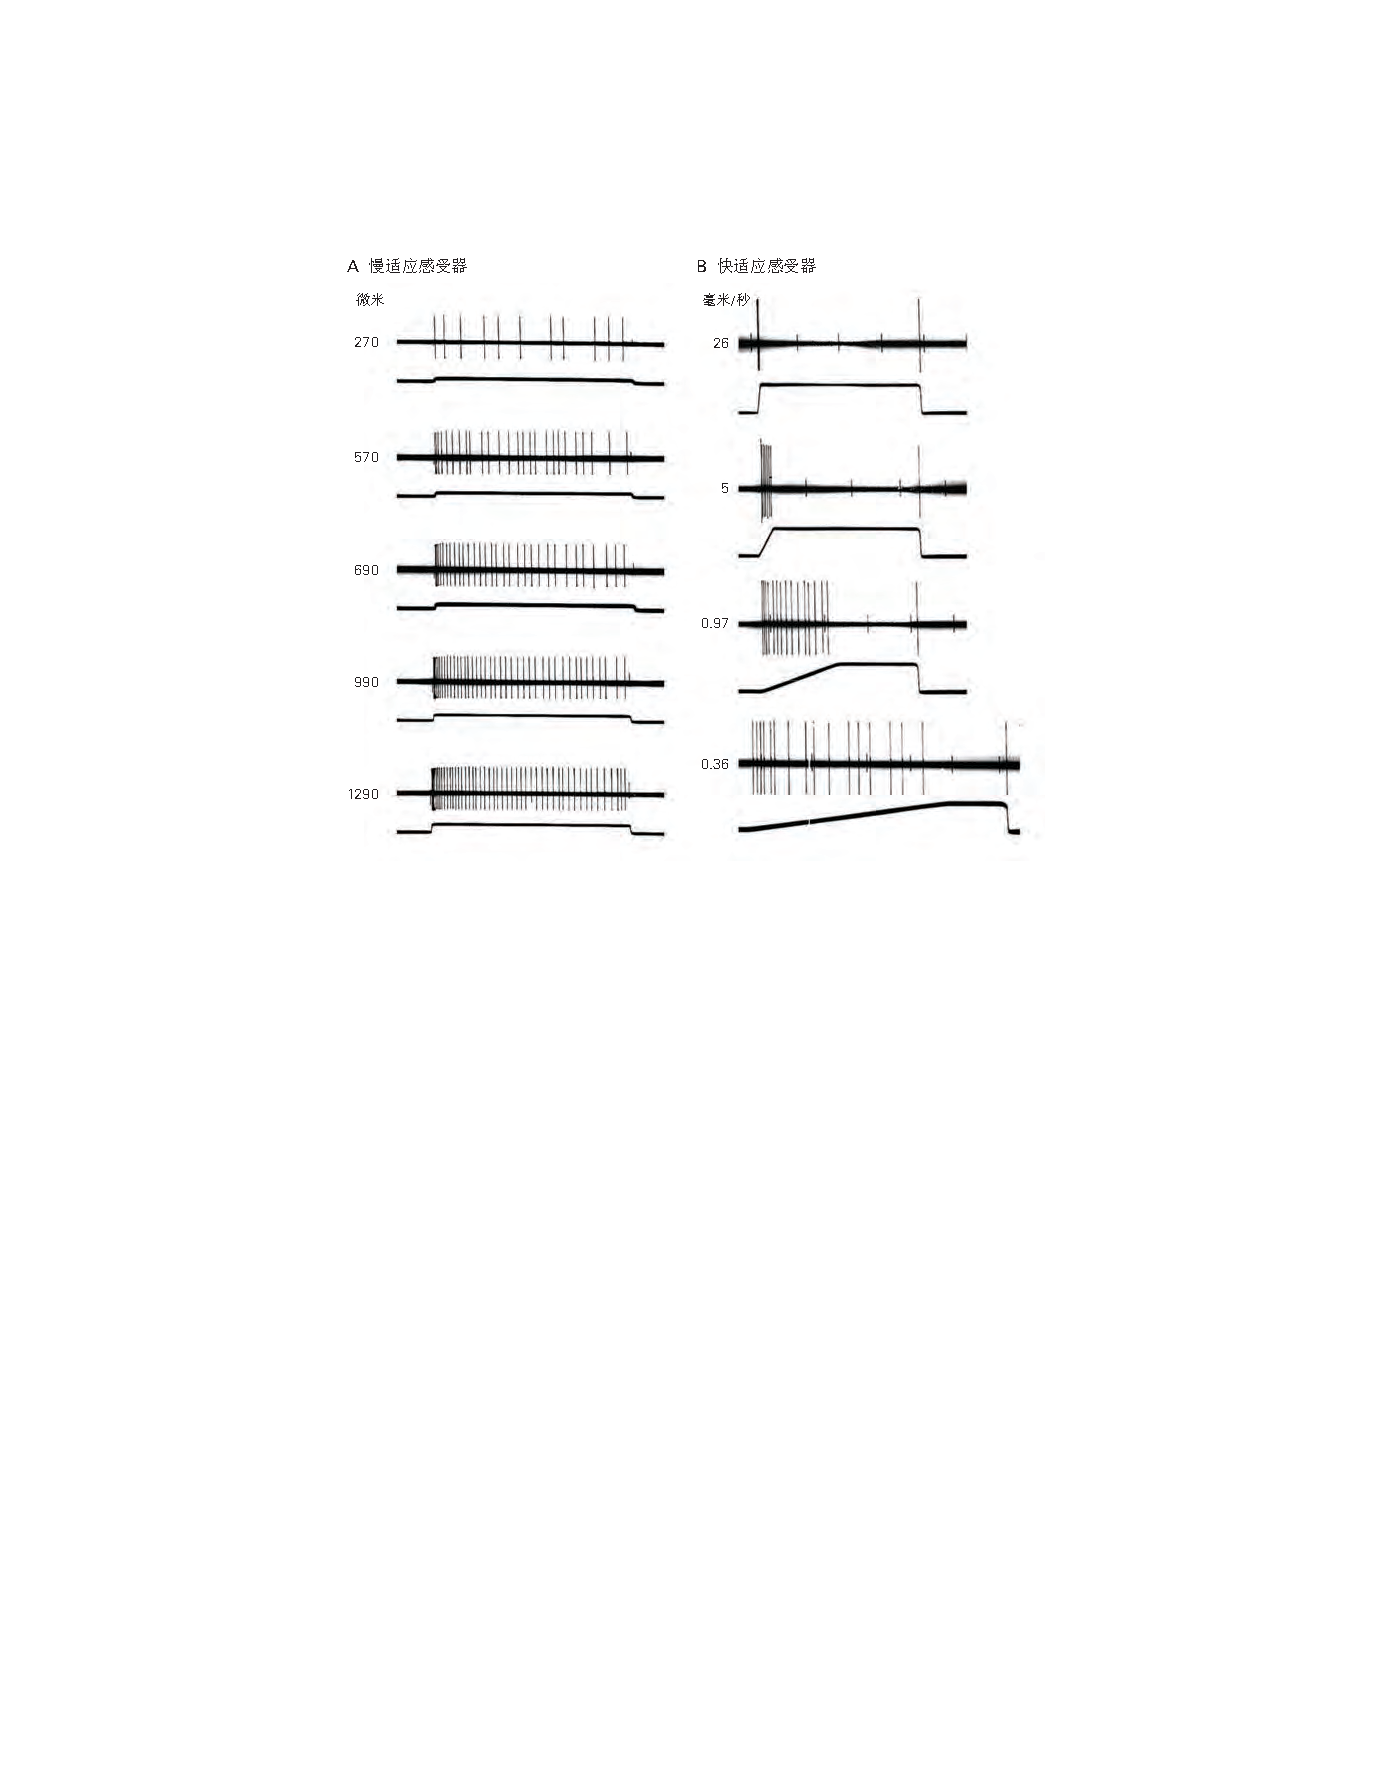
\includegraphics[width=1.0\linewidth]{chap17/fig_17_7}
	\caption{感觉神经元的放电模式传达有关刺激强度和时间进程的信息。
		这些记录说明了两种不同类别的触觉感受器对压入皮肤的探针的反应。 
		刺激幅度和时间过程显示在每对的下方轨迹中; 
		上面的轨迹显示了从感觉神经纤维记录的响应刺激的动作电位。 
		\textbf{A.} 只要对皮肤施加压力,缓慢适应的机械感受器就会做出反应。 
		刺激期间释放的动作电位总数与施加在皮肤上的压力大小成正比。
		皮肤接触开始时的发射率高于稳定压力期间的发射率,因为该受体还会检测压力施加到皮肤上的速度。 
		当探头从皮肤上移开时,尖峰活动停止\cite{mountcastle1966neural}。
		当压力保持在固定幅度时,它是无声的。 
		快速运动会引起短暂的高频尖峰脉冲,而慢速运动会引起持续时间更长的低频尖峰序列\cite{talbot1968sense}。}
	\label{fig:17_7}
\end{figure}


不断变化的刺激的时间特性被编码为放电模式的变化,包括感觉神经元的尖峰间期。
例如,图 \ref{fig:17_7} 中所示的触觉感受器在探针最初接触皮肤时比在保持压力时以更高的速率触发。
当皮肤快速缩进时,尖峰之间的时间间隔比逐渐施加压力时更短。
这些神经元的放电率与压入皮肤的速度和施加的总压力成正比。
在稳定的压力下,发射率减慢到与皮肤压痕成正比的水平(图~\ref{fig:17_7}A)或完全停止(图~\ref{fig:17_7}B)。 
探针缩回后,两个神经元的放电都停止了。


\subsection{感觉神经元的感受野提供有关刺激位置的空间信息}

感觉神经元输入终端在感觉器官中的位置是该神经元传递的特定信息的主要组成部分。 
刺激可以激活感觉神经元的皮肤区域、身体位置、视网膜区域或音域称为它的感受野(图~\ref{fig:17_8})。 
感知到产生感觉的区域称为神经元的感知区域。
两者通常是重合的。


\begin{figure}[htbp]
	\centering
	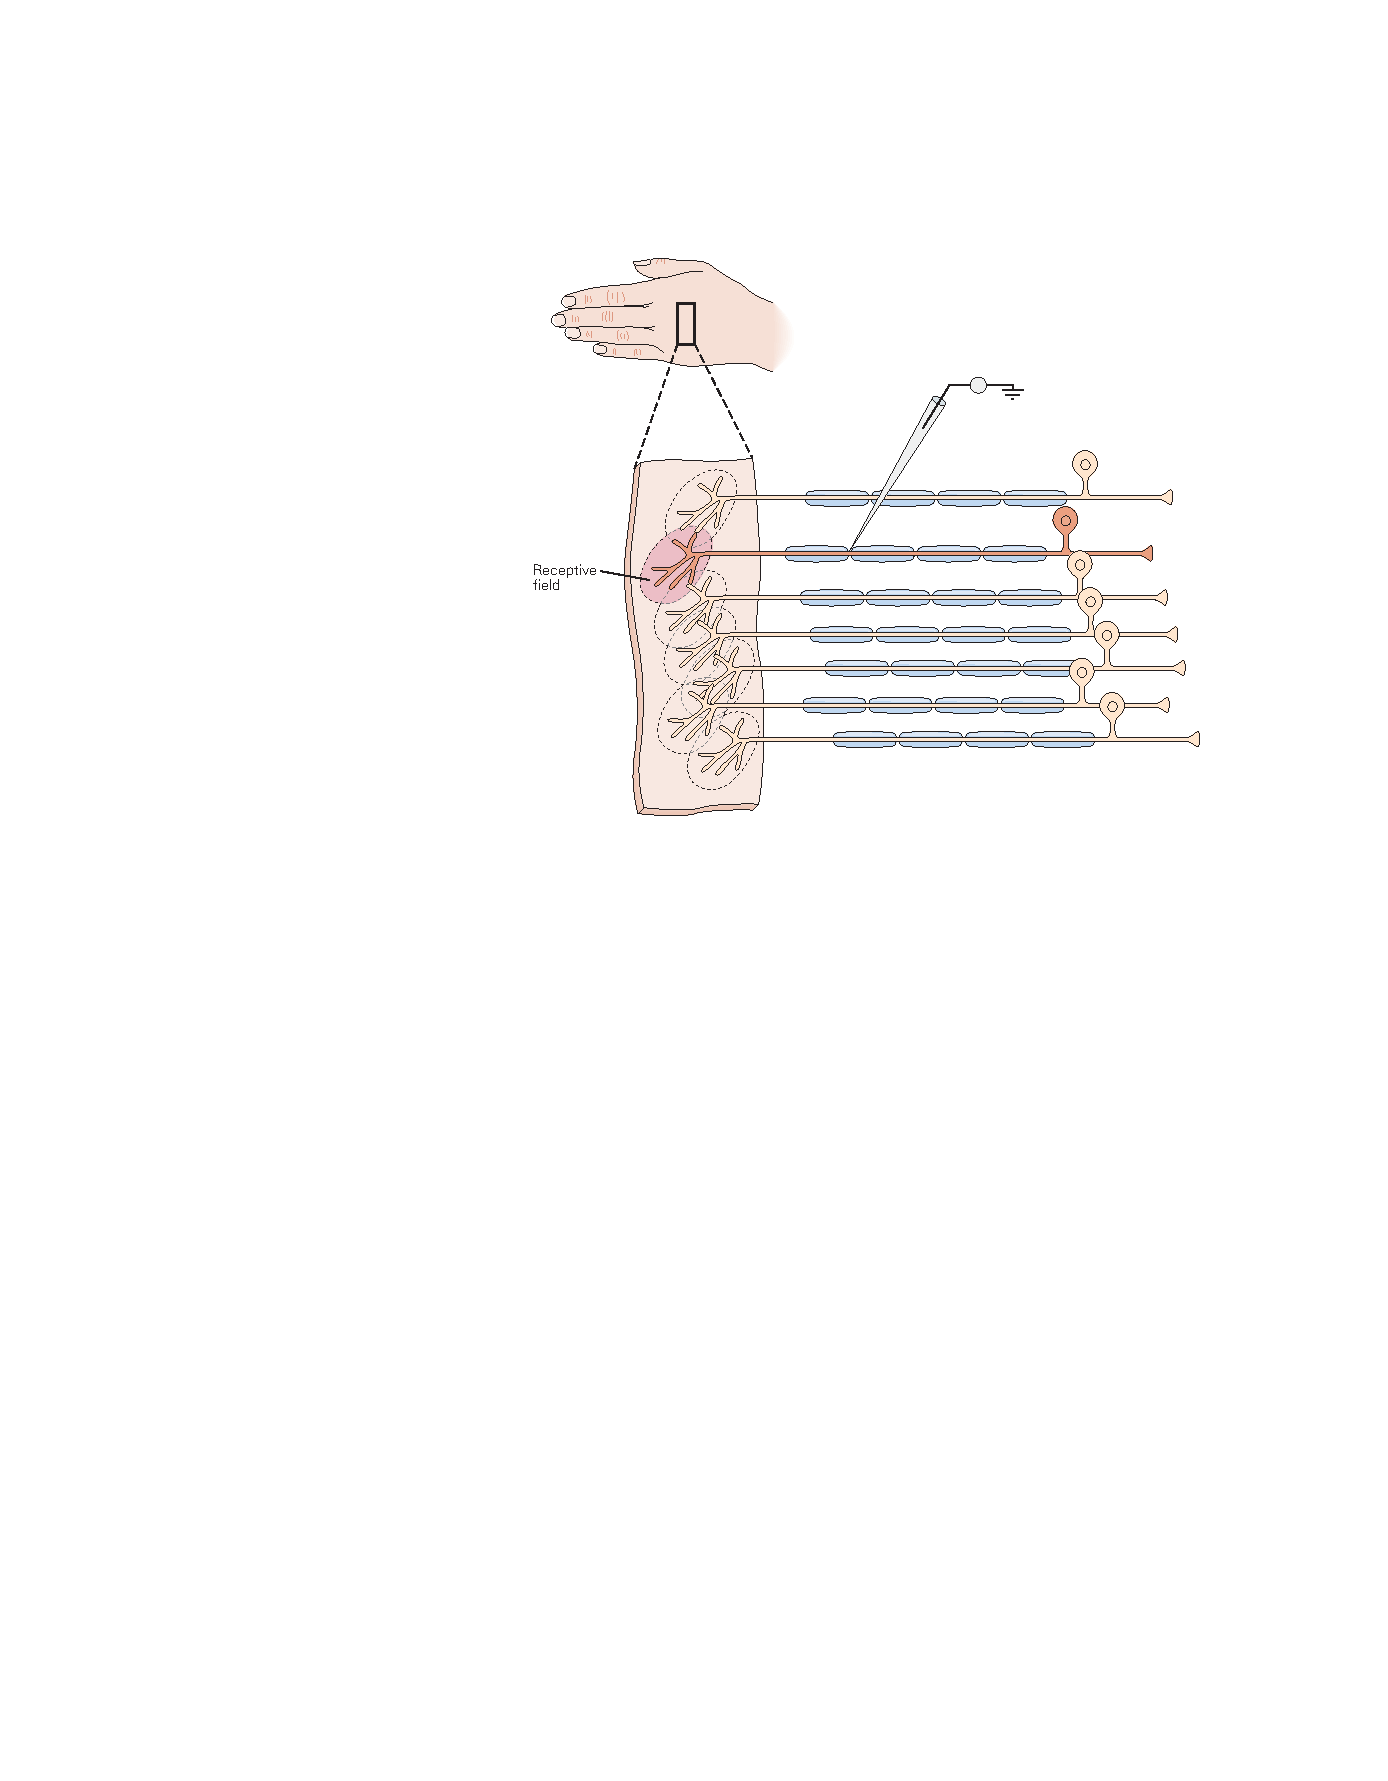
\includegraphics[width=0.7\linewidth]{chap17/fig_17_8}
	\caption{感觉神经元的感受野。
		触敏神经元的感受野表示皮肤区域,轻柔的触觉刺激会在该神经元中唤起动作电位。
		它包括感觉神经纤维的所有接受末梢和末端分支。
		如果用微电极对纤维进行电刺激,则受试者会体验到皮肤上的局部触觉。
		感知到产生感觉的区域称为感知场。
		一块皮肤包含许多重叠的感受野,让感觉在连续扫描中从一个感觉神经元平滑地转移到下一个感觉神经元。
		中枢神经系统中感觉神经元的轴突末端按体表排列,提供了身体神经支配区域的有序图。}
	\label{fig:17_8}
\end{figure}

感受野的维度在感觉系统编码详细空间信息的能力中起着重要作用。 
我们用眼睛看到或拿在手中的物体比单个感觉神经元的感受野大得多,因此会刺激相邻的受体群。 
因此,刺激的大小决定了被激活的受体总数。 
以这种方式,活跃和沉默受体的空间分布提供了刺激大小和轮廓的神经图像。


感觉系统的空间分辨率取决于受体神经元的总数和整个覆盖区域的感受野分布。
具有高密度受体的身体区域的投射神经元,例如代表视网膜中央(中央凹)的视网膜神经节细胞,具有较小的感受野,因为它们接收来自少量双极细胞的输入,每个双极细胞接收 来自一些紧密排列的光感受器的输入。
由于中央凹中的受体密度很高,神经元群传输了非常详细的视觉场景表示。
视网膜周边的神经节细胞具有更大的感受野,因为受体密度要低得多。
这些神经节细胞的树突从更广泛的视网膜区域接收信息,从而将光强度整合到更大范围的视野中。
这种安排产生了视觉场景的不太详细的图像(图~\ref{fig:17_9})。
同样,最常用于触摸物体的身体部位是手。
毫不奇怪,触摸的机械感受器集中在指尖,手上的感受野比手臂或躯干上的感受野小。


\begin{figure}[htbp]
	\centering
	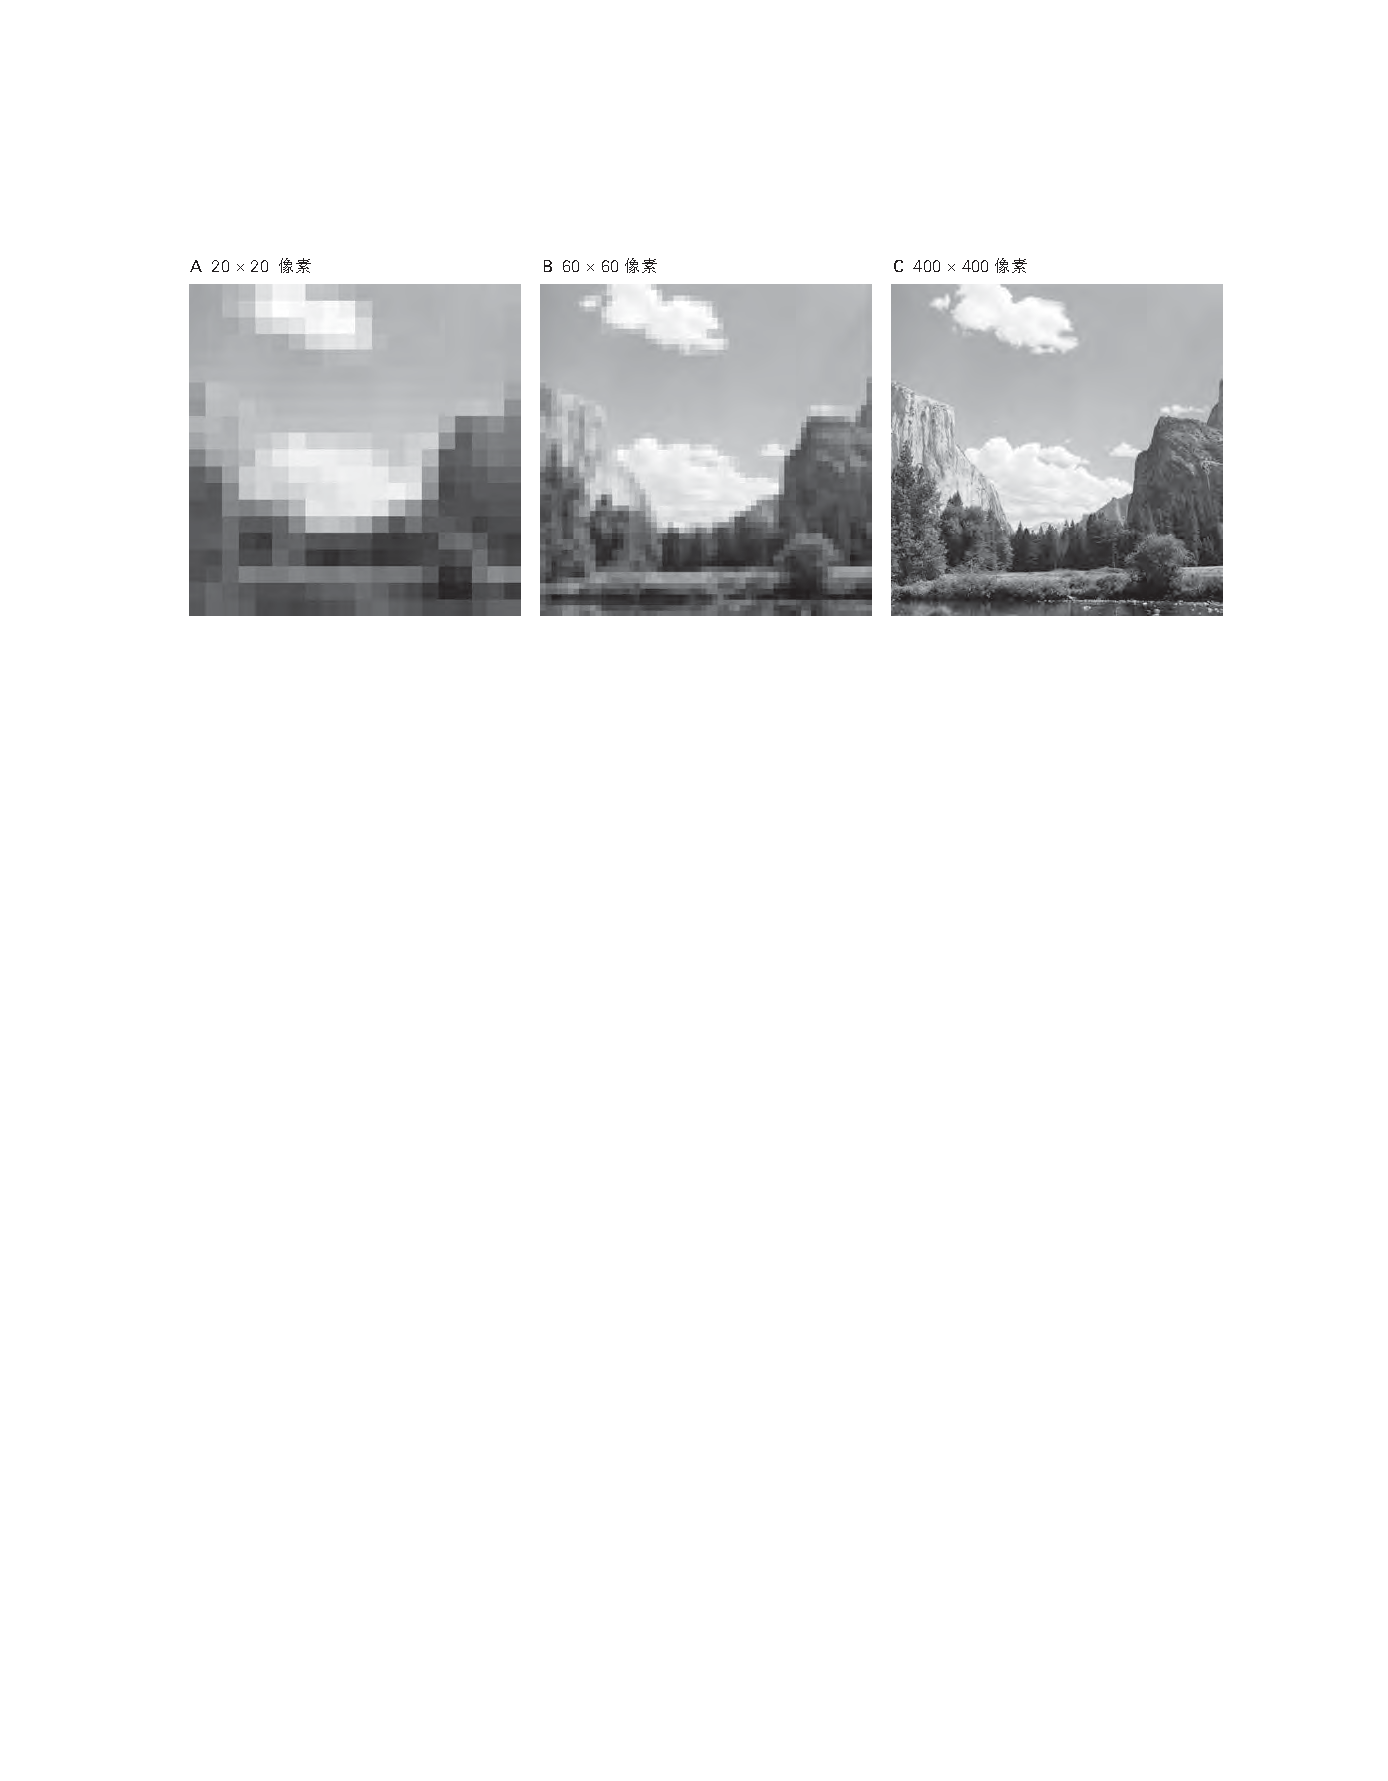
\includegraphics[width=0.7\linewidth]{chap17/fig_17_9}
	\caption{场景和物体的视觉分辨率取决于调节图像的光感受器的密度。
		细节的分辨率与单个神经元的感受野面积呈负相关。
		这些图像中的每个正方形或像素代表一个感受野。
		每个像素中的灰度级与相应感受野中的平均光强度成正比。
		如果有少量神经元,并且每个神经元跨越图像的大面积,则结果是场景 (A) 的非常示意性表示。 
		随着神经元密度的增加,每个感受野的大小减小,空间细节变得更加清晰(B,C)。
		空间分辨率的提高是以传输信息所需的大量神经元为代价的。}
	\label{fig:17_9}
\end{figure}



\section{中枢神经系统回路完善感官信息}

感觉神经元的中央连接决定了该神经元的信号如何影响我们的感官体验。 
例如,耳蜗神经纤维中的动作电位会引起音调感觉,无论它们是由作用于毛细胞的声波还是通过神经假体的电刺激引发的。


将刺激分成其组成部分,每个组成部分由一种单独类型的感觉受体或投射神经元编码,是感觉处理的初始步骤。 
这些组件通过大脑中的神经网络集成到对象或场景的表示中。 
这个过程允许大脑从许多感受器的详细输入中选择一个物体、人、场景或外部事件的某些抽象特征。 
结果,在大脑中形成的表示可能会增强当前重要特征的显着性,同时忽略其他特征。 
从这个意义上说,我们的感知不仅是环境事件的反映,而且是心灵的建构。


我们如何体验主要感受器报告的感觉也需要修改或学习。 
例如,最初厌恶的气味和味道会随着时间的推移变得有吸引力,因为熟悉或环境或联想发生变化。 
如果一位受人尊敬的棒球运动员随后穿着对手球队的制服出现,那么他的照片所引起的愉悦可能会转化为蔑视。


在中枢神经系统感觉信息处理的早期阶段,每一类外周受体都为专用于一种感觉方式的中继核中的神经元簇提供输入。 
也就是说,每种感觉方式都由连接到特定类别受体的一组中枢神经元表示。 
这样的整体被称为感觉系统,包括体感、视觉、听觉、前庭、嗅觉和味觉系统(见表~\ref{tab:17_1})。


大脑已经进化到可以处理和响应这些丰富的感官信息。 
人脑中感觉、认知和运动系统的激活可以通过\textit{功能性磁共振成像}技术实时可视化。 
Maurizio Corbetta、Marcus Raichle 及其同事发现,在“静息”状态下,大脑区域的\textit{血氧水平依赖性}信号的低频 (0.01–0.1 Hz) 分量会发生相干波动 具体行为。 
图~\ref{fig:17_10}~突出显示了大脑区域的三个功能专门化网络,这些区域响应听觉(红色)、躯体运动(绿色)和视觉(蓝色)输入。 
其他领域是多感官的,整合了来自几种不同模式的信息。 
在没有直接感觉刺激或运动任务执行的情况下,这些网络的自发相关性表明,静息状态感觉或运动网络内的兴奋性可能表示准备好为未来的感觉或行动处理信息。 
局部脑损伤后的感觉、认知或运动功能缺陷可能不仅是由于某一特定区域或节点的损伤,还可能是由于包含该节点的回路或回路中断所致。


\begin{figure}[htbp]
	\centering
	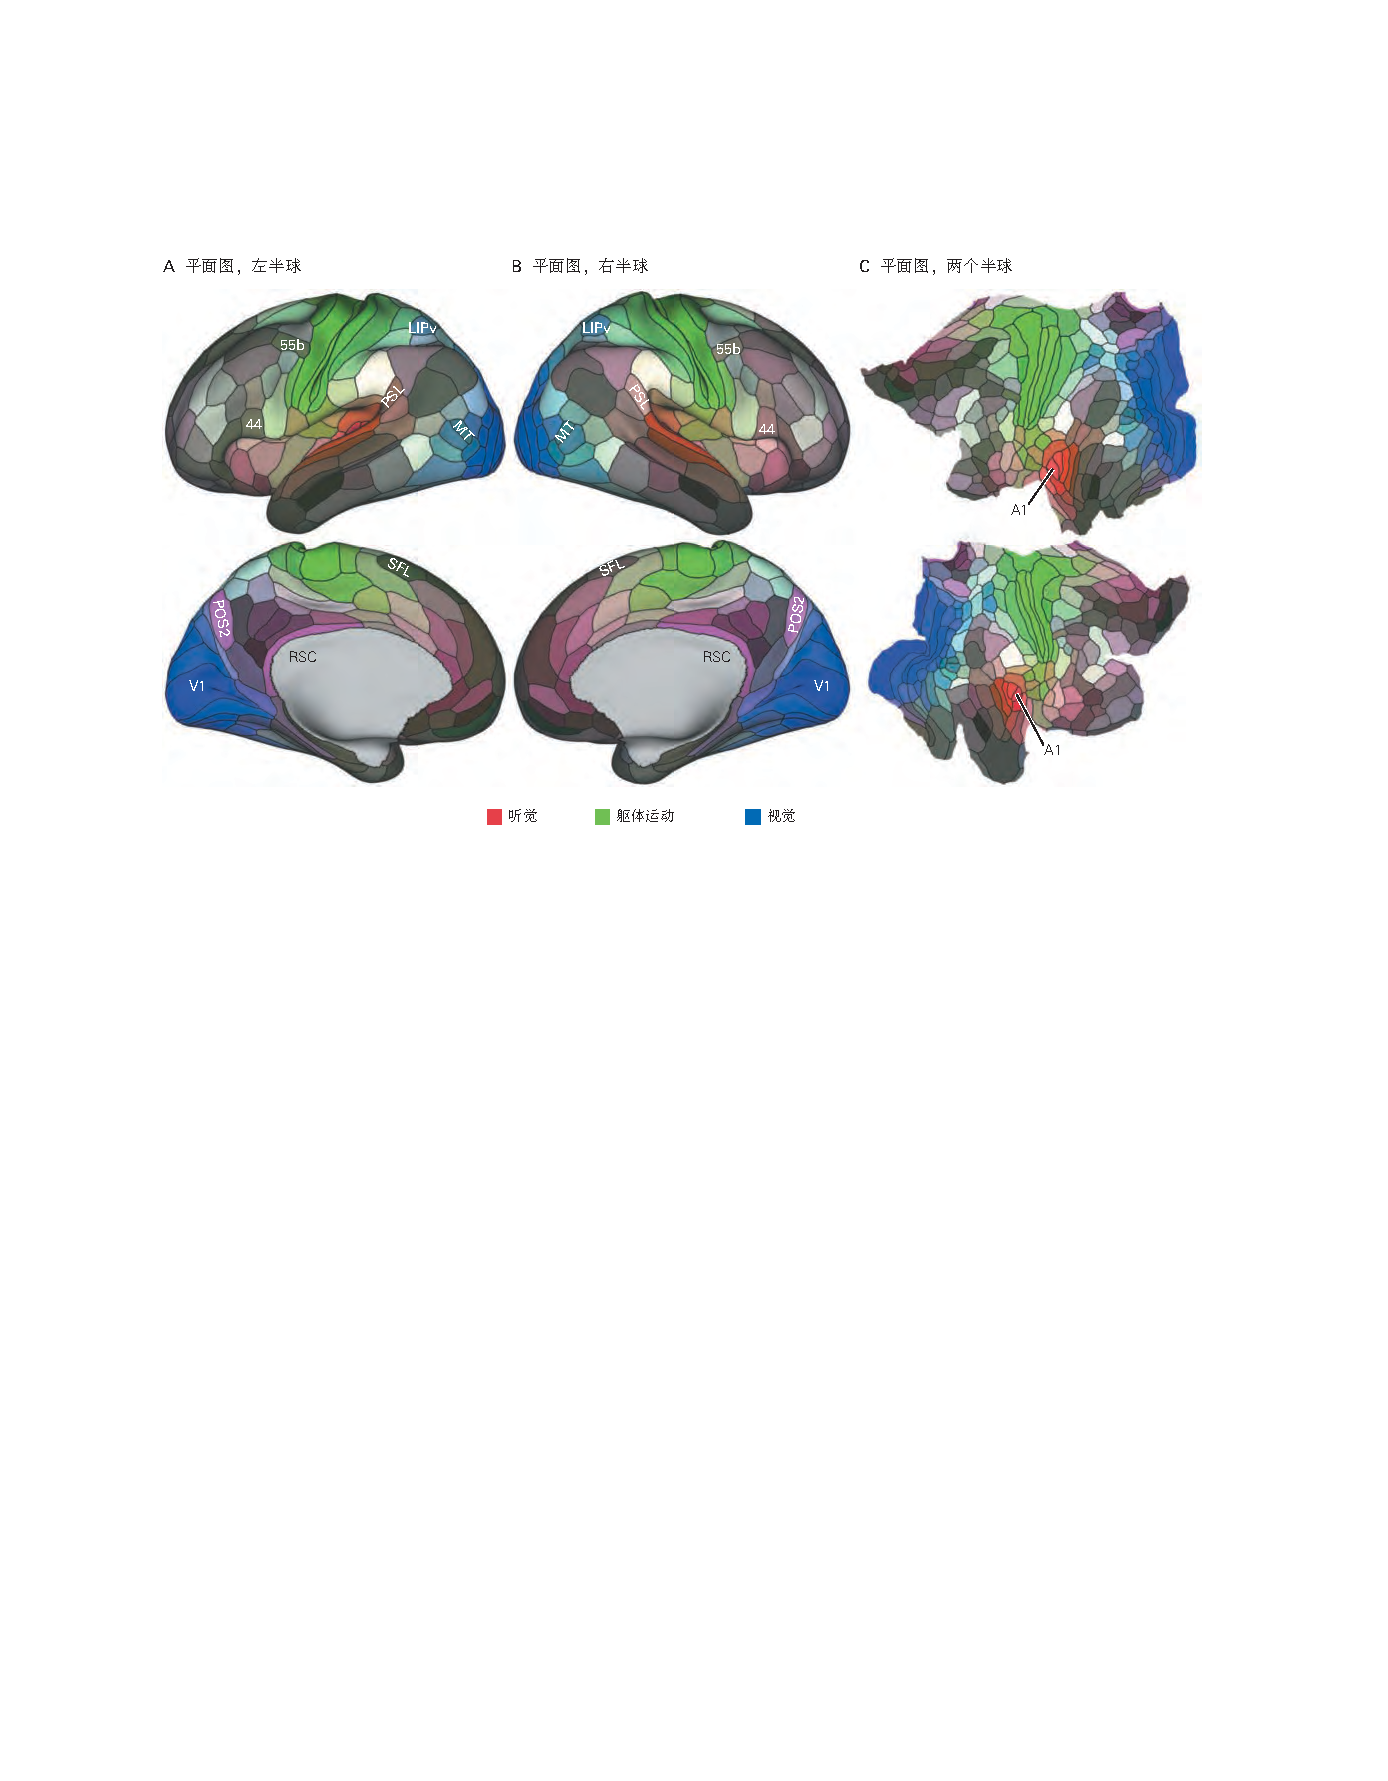
\includegraphics[width=0.7\linewidth]{chap17/fig_17_10}
	\caption{人脑的不同区域处理个人感觉方式、多感觉系统、运动活动或认知功能的信息。
		人类连接组计划主要基于各种\textit{功能性磁共振成像}技术和神经解剖学,将人类大脑皮层划分为 180 个功能区域。 
		早期听觉区(红色)、体感和运动区(绿色)和视觉区(蓝色)以原色阴影显示。
		混合颜色表示多感官区域:视觉和体感/运动(蓝绿色、LIPv、MT); 或视觉和听觉(粉色到紫色、POS2、RSC)。
		语言网络包括两个半球的区域 55b、44、SFL 和 PSL。
		灰度区域服务于认知功能; 它们包括反相关的“任务正向”(浅色阴影)和“默认模式”(深色阴影)网络。 
		这些地图显示位于表面回旋和相邻皮层沟内的大脑区域。
		注意两个半球之间大脑组织的相似性\cite{glasser2016multi}。
		数据可在 https://balsa 获取。 wustl.edu/study/RVVG。
		\textbf{A.} 左半球的膨胀图。 上图是侧视图,下图是中视图。
		\textbf{B.} 右半球的相似地图。 
		\textbf{C.} 扁平化的地图显示了两个半球的功能组织(左上,右下)。 
		(缩写:A1,初级听觉皮层;LIPv,外侧顶内区,腹侧部分;MT,颞中区;POS2,顶枕沟区 2;PSL,外侧裂语言区;RSC,脾后复合体;SFL,额上语言区 ;V1,初级视觉皮层;55b 区,新发现的语言区;44 区,布罗卡区的一部分。)}
	\label{fig:17_10}
\end{figure}


感觉通路中的突触提供了修改来自受体的信号的机会。 
中继核中的大多数神经元从许多突触前神经元接收会聚兴奋性输入(图~\ref{fig:17_11}A),整合这些输入,将它们与抑制和自上而下的信号结合,并将处理后的信息传输到更高的大脑区域。 
\textit{霍勒斯·巴洛}提出,感觉系统展示了高效的编码,其中包括重新编码感觉信息的感觉中继,以减少它们的冗余,但丢失的信息相对较少。 
同样,每个受体神经元都会激发多个突触后中继神经元。


\begin{figure}[htbp]
	\centering
	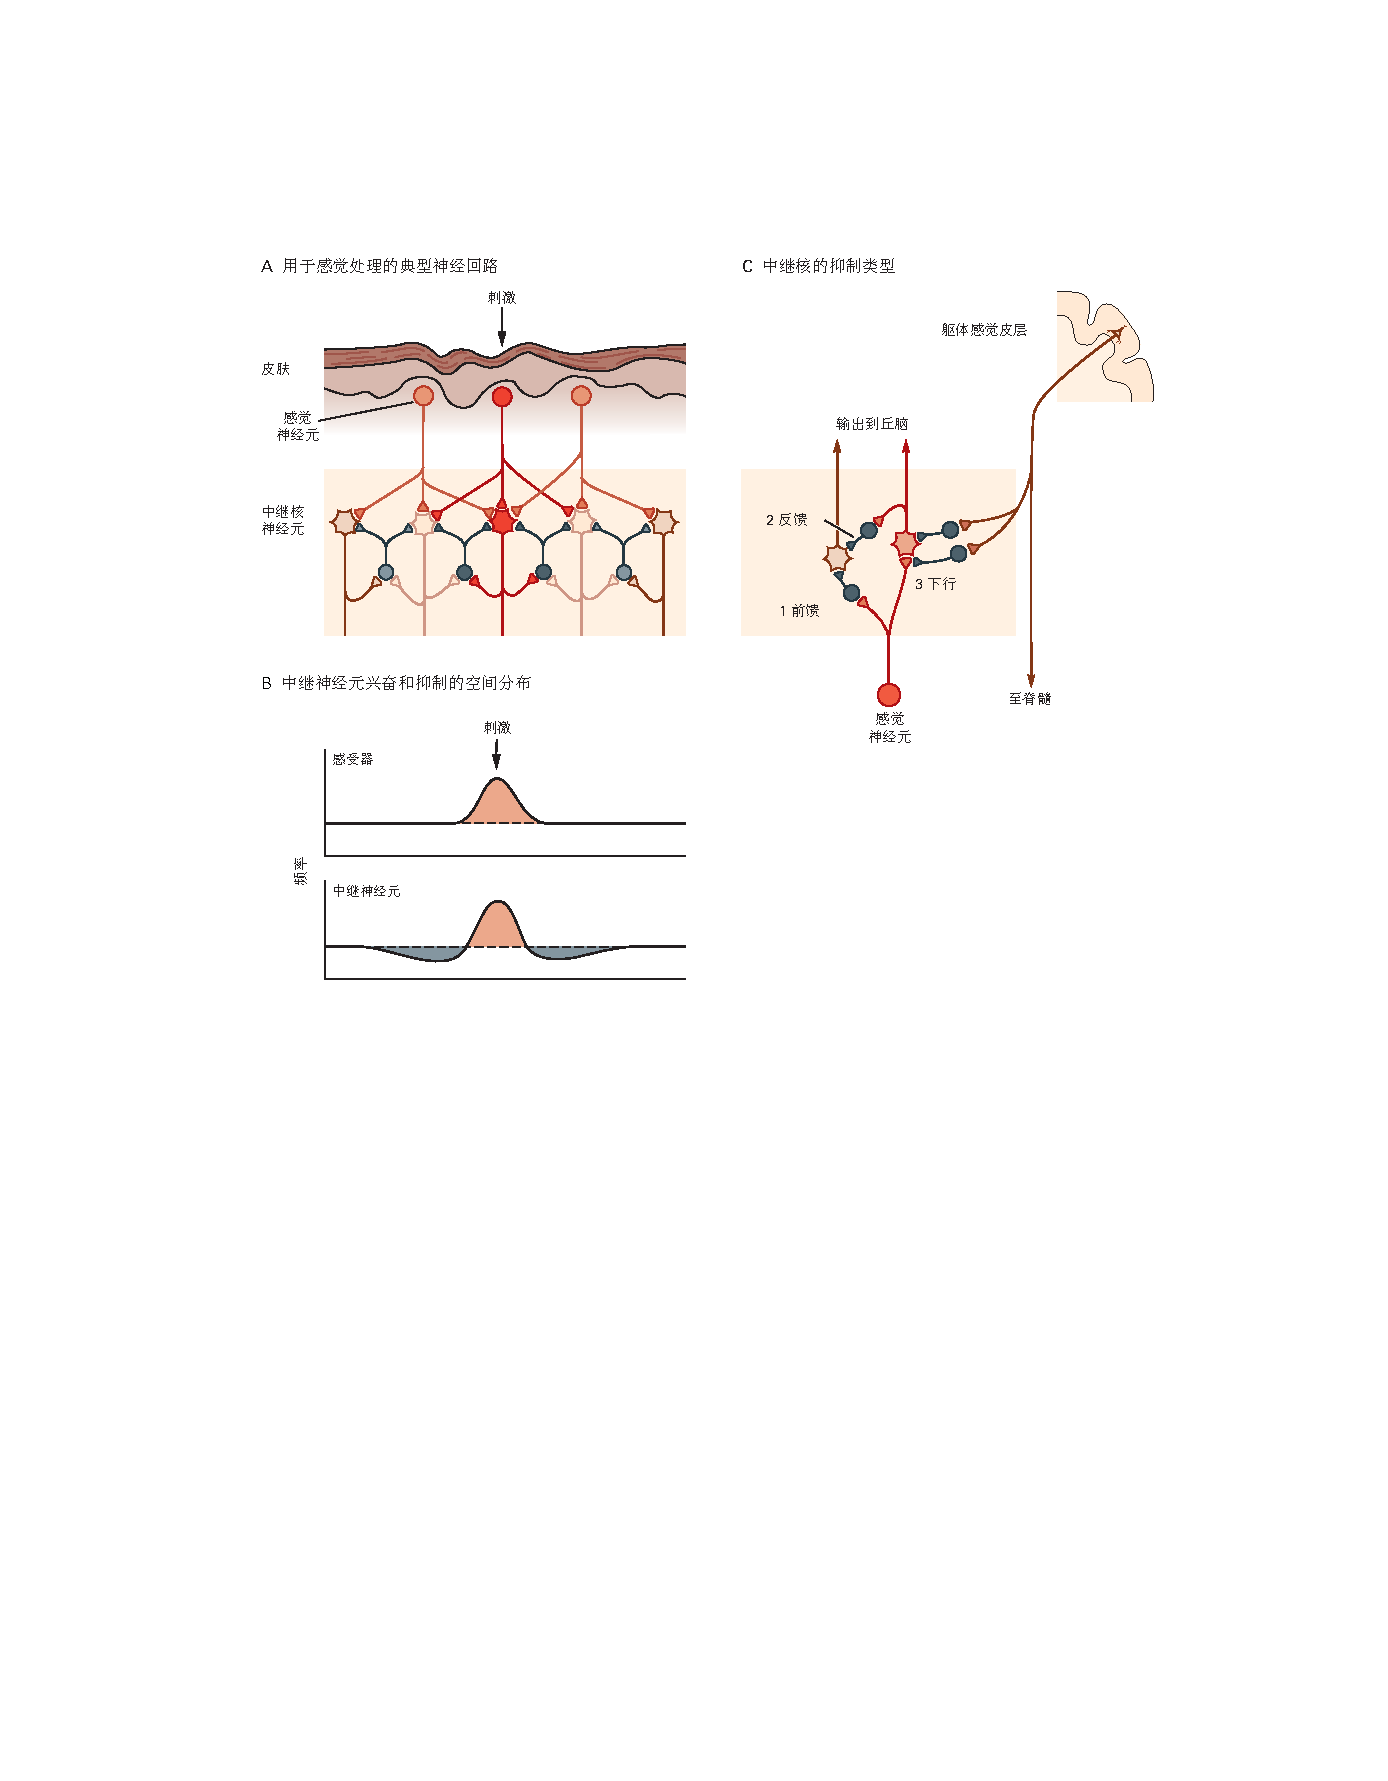
\includegraphics[width=0.7\linewidth]{chap17/fig_17_11}
	\caption{感觉系统中的中继神经元整合了形成刺激信息的各种输入。 
		\textbf{A.} 感觉信息通过分级处理网络在中枢神经系统中传输。 
		由皮肤刺激引发的神经信号到达脑干和丘脑中继核中的一大群突触后神经元,并且在突触后细胞阵列中心的神经元(红色神经元)中最强\cite{biederman2013human}。
		\textbf{B.} 由局部中间神经元(灰色)介导的抑制(灰色区域)将兴奋(橙色区域)限制在刺激最强的中继神经元阵列的中央区域。 
		中继核内的这种抑制模式增强了强烈和弱刺激的中继神经元之间的对比。 
		\textbf{C.} 中继核中的抑制性中间神经元由三种不同的兴奋途径激活。 
		1. 前馈抑制由终止于抑制性中间神经元的感觉神经元的传入纤维启动。 
		2. 反馈抑制是由核输出通路中神经元的循环侧支轴突启动的,它投射回源核中的中间神经元。 
		中间神经元反过来抑制附近的输出神经元,在中继核中形成清晰的兴奋和抑制活动区域。 
		通过这种方式,最活跃的中继神经元会减少相邻的、不太活跃的神经元的输出,从而确保两个或多个活跃神经元中只有一个会发出信号。 
		3. 下行抑制是由大脑皮层等其他大脑区域的神经元启动的。 
		下行命令允许皮层神经元控制感觉信息的传入中继,提供一种机制,注意力可以通过该机制选择感觉输入。}
	\label{fig:17_11}
\end{figure}


会聚兴奋网络为输入的空间求和提供了一种机制,加强了功能重要性的信号。 
如何使用此类回路的一个示例是检测来自多个附近位置而非其他位置的同步输入,从而为中枢神经元的定向调整提供了第一步。 
中继神经元也与其相邻神经元相互连接,形成可放大感觉信号的循环兴奋性连接。 
这种循环网络也是人工神经网络用来对感觉模式进行分类的一些深度学习算法的一个特征。


中继神经元的感受野也受到抑制性输入的影响。 
感受野的抑制区域为增强刺激之间的对比提供了重要机制,赋予感觉系统额外的能力来解析空间细节。 
抑制性中间神经元调节中继核中神经元的兴奋性,从而调节传输到网络更高级别的感觉信息量(图~\ref{fig:17_11}B)。 
抑制回路也可用于抑制目标导向行为期间的无关信息,从而将注意力集中在与特定任务相关的输入上。 
此外,抑制网络允许刺激的上下文修改由该刺激引起的兴奋强度,这是一个称为正常化的重要过程。


与外周受体相比,中枢神经元对感觉刺激的反应在不同的试验中变化更大。 
中枢感觉神经元在刺激前后以及没有刺激时也会不规则地放电。 
诱发的中枢反应的可变性是几个因素的结果:
受试者的警觉状态、注意力是否参与(图~\ref{fig:17_12})、该刺激的先前经验以及类似刺激最近激活的通路。 
同样,刺激呈现的背景、主观意图、可能需要反馈的运动计划或神经元膜电位的固有振荡都可以修改传入的感觉信息。


\begin{figure}[htbp]
	\centering
	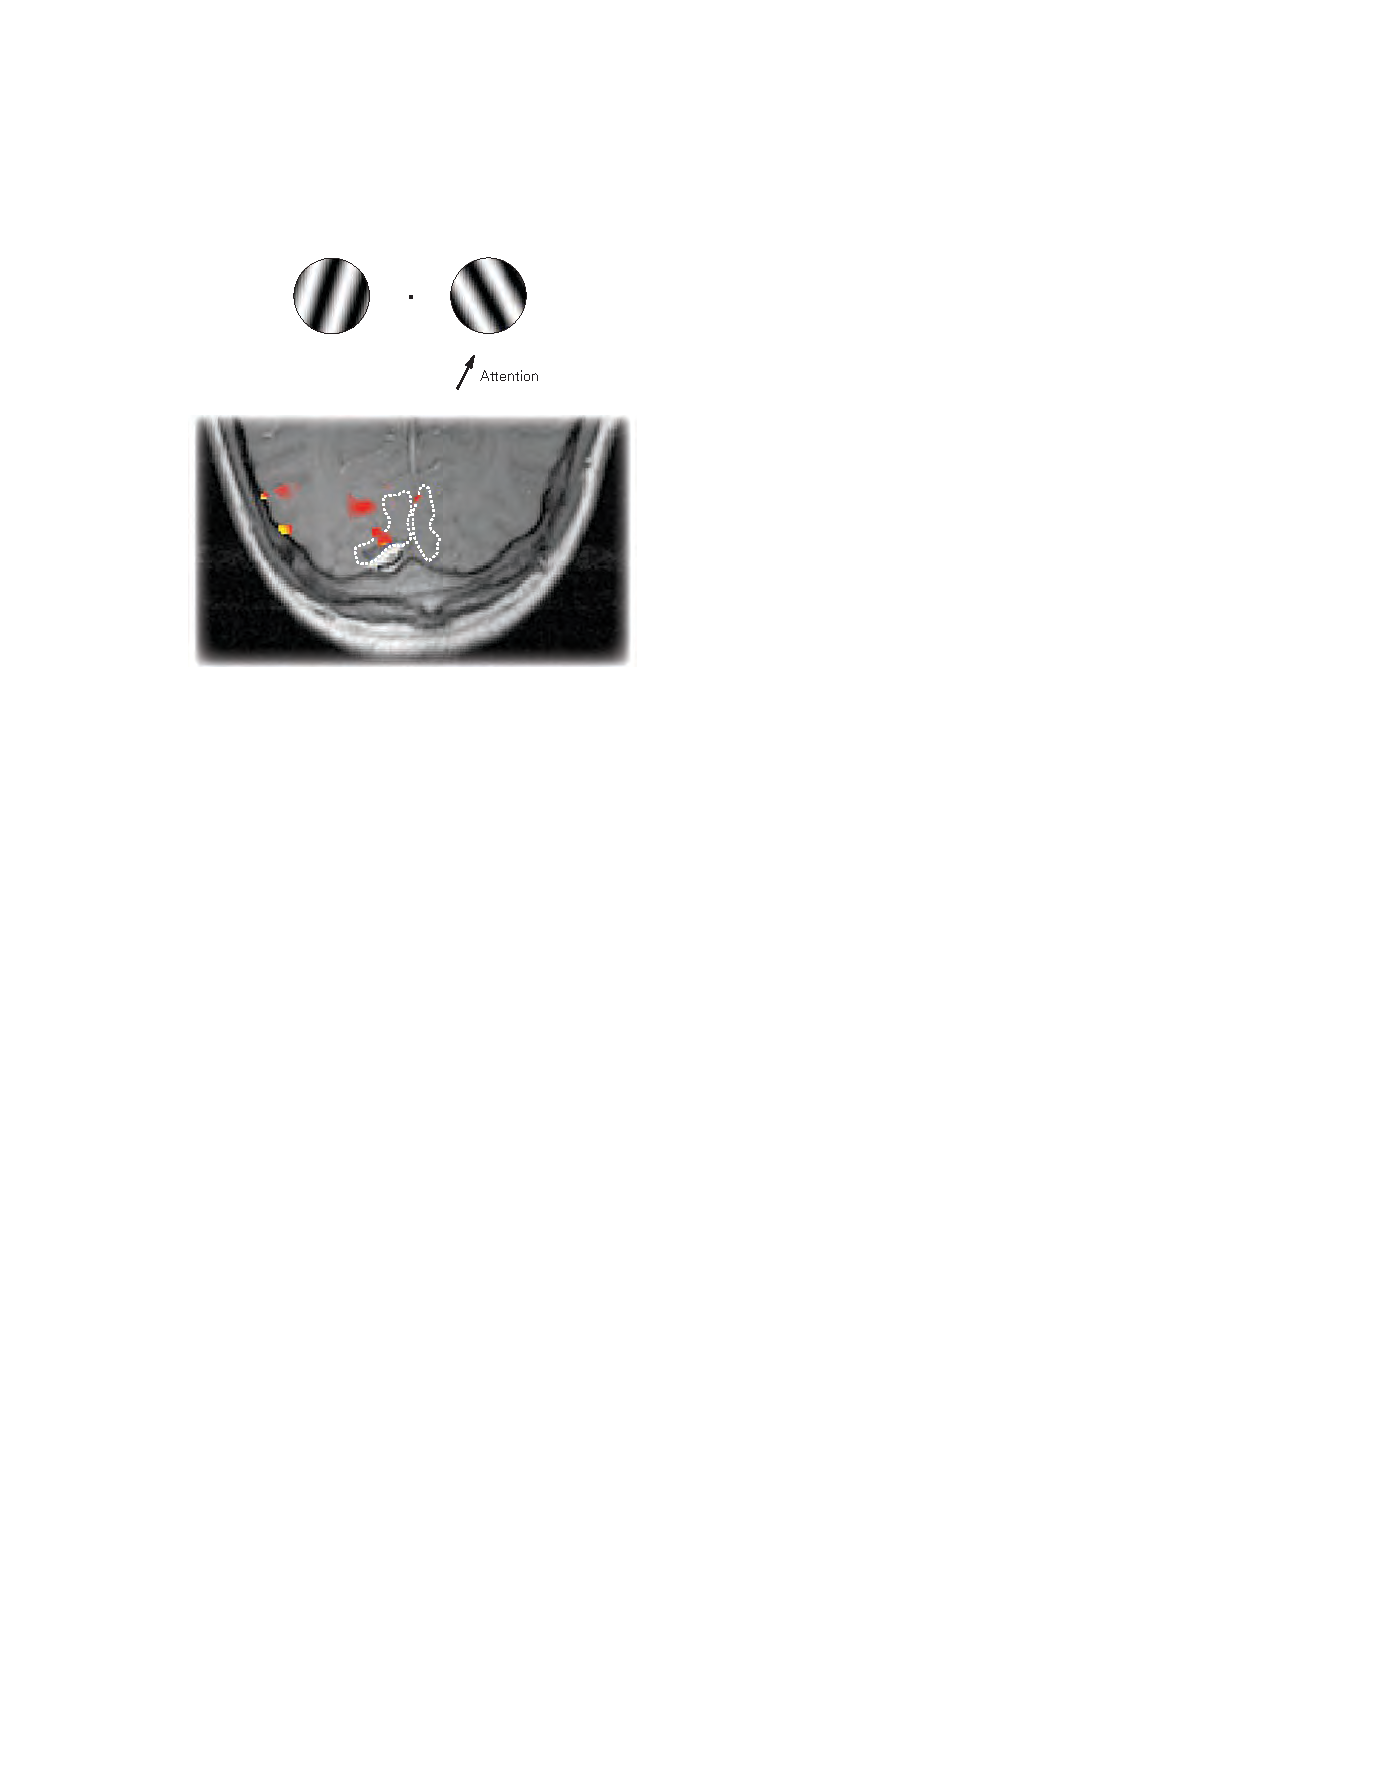
\includegraphics[width=0.5\linewidth]{chap17/fig_17_12}
	\caption{注意视觉刺激会改变视觉皮层区域神经元的反应。 
		当我们注意刺激时,我们会选择某些感官输入进行认知处理,而忽略或抑制其他信息。
		本研究使用\textit{功能性核磁共振成像}来测量视觉刺激注意力对人类\textit{初级视觉皮层}神经响应的影响(大脑解剖切片上的白色虚线,下图)。 
		移动光栅刺激(上图)同时出现在左右视野中,而受试者盯着中央注视点(黑点)。 
		受试者执行运动辨别任务,注意(不移动眼睛)两个定向光栅之一。 
		当刺激出现在右侧视野时,左半球的神经活动(红色)显着增加,但右半球没有,即使双眼都受到刺激。 
		当受试者注意左侧视野中的光栅时,右侧\textit{初级视觉皮层}会出现类似的活动焦点,而左侧半球的活动会下降(未显示)\cite{gandhi1999spatial}。}
	\label{fig:17_12}
\end{figure}


\subsection{受体表面在每个感觉系统的早期阶段都以地形图表示}

感觉投射神经元的轴突以有序的方式终止于大脑中,并保持其在受体片中的空间排列。 
皮肤相邻区域的感觉神经元投射到中枢神经系统的相邻神经元,并且这种感受野的地形排列在整个早期体感通路中得到保留。 
因此,大脑中的每个主要感觉区域都包含感觉器官的地形图、空间组织图。 
这种地形扩展到感官系统的所有层次。 
在这些地图中,特异性——神经元最窄地调整到的特性——为大脑该区域的功能组织提供了线索。


在体感、视觉和听觉系统的第一个和随后的中继核中,相邻的神经元分别代表身体、视网膜和耳蜗的相邻区域。 
因此,这些细胞核的组织被称为体细胞、视网膜细胞或音质细胞。 
听觉系统中的核是音调性的,因为内耳的耳蜗毛细胞排列成在细胞与细胞之间产生频率敏感度的有序转移(图~\ref{fig:26_2})。 
大脑皮层初级感觉区的神经元维持刺激的这些特定位置特征,这些早期皮层区域的功能图同样是躯体、视网膜或音质。


感觉信息在到达与认知和行动有关的大脑区域之前,通过包括多个层次的大脑皮层在内的层级通路连续流动。
形成通知这些区域的感知需要整合较低级别的输入,这些输入仅报告来自感觉器官小区域的信息。
大脑皮层中的神经元专门用于整合并因此检测刺激的特定特征,而不仅仅是它们在感觉器官中的位置。
据说这样的神经元被调谐到以感觉受体集合为代表的组合刺激特征。
这些神经元优先响应刺激特性,例如边缘的方向(例如,特定受体组的同时激活)、运动方向或频率的音调序列(受体激活的时间模式)。
中枢听觉神经元对频率的选择性较低,而对某些声音的选择性较高。
例如,一些神经元特定于同一物种成员的发声。
在皮层处理的每个后续阶段,随着神经元越来越不关心刺激的描述性特征,而越来越关心行为重要性的特性,刺激的空间组织逐渐丢失。
这些中枢感觉转换的详细信息将在随后描述特定感觉系统的章节中介绍。



\subsection{感觉信息在大脑皮层的平行通路中被处理}

分布式空间编码在感觉系统中普遍存在有两个原因。 
首先,它利用了神经系统的并行架构。 
大脑皮层的每个初级感觉区大约有1亿个神经元,神经活动可能的组合模式数量远远超过宇宙中原子的数量。 
其次,每个神经元编码刺激的强度和时间以及它在受体片中的位置。 
只有当它的许多兴奋性突触接收到动作电位而大多数抑制性突触没有接收到动作电位时,它才会触发,触发是为了响应特定的刺激模式而不是其他模式。 
由于许多皮层神经元接收来自 1 千到 1 万个突触的输入,因此信息编码潜力巨大。


Mortimer Mishkin 和 Leslie Ungerleider 在 1980 年代早期对视觉皮层通路进行的生理学和解剖学综合研究产生了对皮质特征检测的最重要见解之一。 
他们发现到达主要视觉区域的感觉信息分为两条平行通路。


一条路径携带图像分类所需的信息,而另一条路径传送立即采取行动所需的信息。 
识别物体是什么的视觉特征通过腹侧通路传输到颞叶,最终传输到海马体和内嗅皮层。 
关于物体所在位置、大小和形状以及如何获取和使用物体的视觉信息通过更靠背的通路传输到顶叶,并最终传输到额叶皮层的运动区(图~\ref{fig:17_13})。


\begin{figure}[htbp]
	\centering
	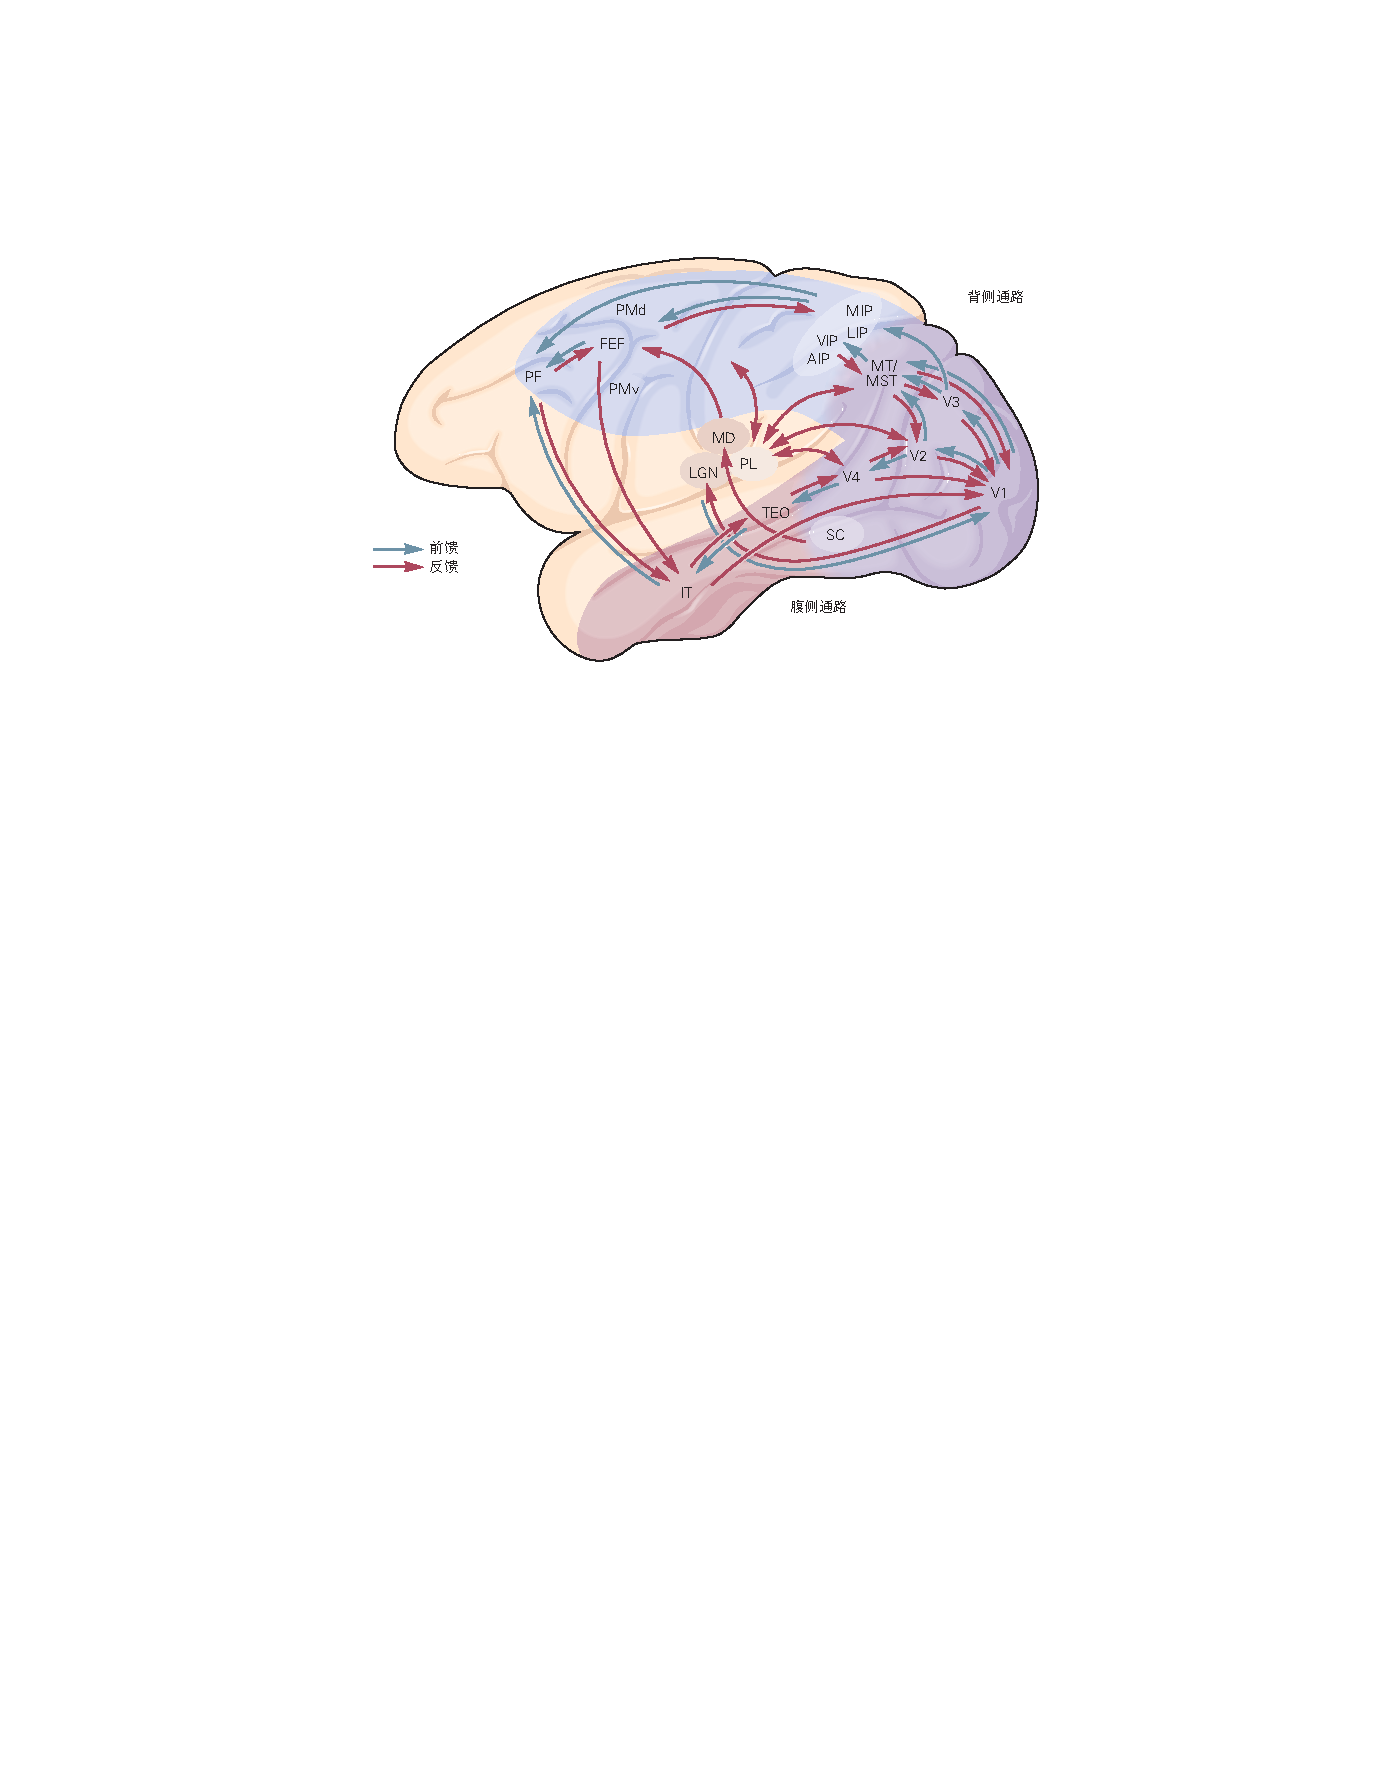
\includegraphics[width=1.0\linewidth]{chap17/fig_17_13}
	\caption{视觉刺激由大脑皮层中的串行和并行网络处理。 
		当你阅读这篇文章时,字母的空间模式通过连续的突触链接发送到大脑皮层,这些突触链接包括光感受器、视网膜双极细胞、视网膜神经节细胞、丘脑\textit{外侧膝状体核}细胞和\textit{初级视觉皮层}神经元。 
		在大脑皮层内,逐渐分化为连续的处理区域,称为腹侧和背侧流,这些区域既不完全连续也不完全平行。 
		颞叶中的腹侧流(红色阴影)分析和编码有关视觉场景和其中物体的形式和结构的信息,将这些信息传递到海马旁皮层(未显示)和前额叶皮层。
		顶叶(蓝色阴影)中的背侧流分析和表示有关刺激位置和运动的信息,并将这些信息传递到控制眼睛、手和手臂运动的额叶皮层的运动区域。
		这些区域之间的解剖学联系是相互的,涉及前馈和反馈回路。
		重叠区域(紫色)表明两条通路都源自\textit{初级视觉皮层}中的同一来源。
		与丘脑和中脑皮层下结构的连接在图~\ref{fig:21_7}B 中定义。 (缩写:V1、V2、V3 和 V4,枕骨视觉区;MT,中颞叶;MST,内侧上颞叶;AIP、VIP、LIP 和 MIP,前部、腹侧、外侧和内侧顶内;TEO,颞叶- 枕骨;IT,颞下;PMd 和 PMv,背侧和腹侧前运动;FEF,额叶视野。)\cite{albright2002contextual}}
	\label{fig:17_13}
\end{figure}


腹侧和背侧流在其他感觉系统中也很明显。 
在听觉系统中,来自语音的声学信息被传输到颞叶的韦尼克区,该区在语言理解中起着重要作用,并传输到额叶皮层的布罗卡区,该区参与语音产生。 
在体感系统中,有关物体大小和形状的信息被传输到顶叶皮层的腹侧区域以进行物体识别。 
有关物体大小、重量和质地的触觉信息也会传送到后顶叶和额叶运动区,这些区域需要规划物体的处理。


感觉信息的腹侧和背侧流也有助于记忆的两种主要形式:语义(也称为显性)记忆,我们用来谈论物体或人,以及程序性(也称为隐性)记忆,我们用来与物体交互 、人员或直接环境。


腹侧流信息生成我们用来识别和分类人、地点和物体(例如球体、砖块和汽车)的名词。 
背流信息激发动词,使动词能够根据感官输入和主观意图执行动作,例如抓握、举起或驾驶。



\subsection{来自大脑的反馈通路调节感觉编码机制}

感觉系统不是简单的自动装配线,它将环境事件(例如,光、声音、气味)的零散神经表征重新组合成更连贯的感知。 
我们可以极大地控制自己的感觉和知觉体验,甚至是我们有意识的注意力。


我们可以在某种程度上控制哪些感觉到达我们的意识。 
例如,我们可能会通过看电视来转移注意力,以摆脱脚踝扭伤带来的疼痛。 
通过突然将注意力转移到身体的某个部位,例如左手的手指,您可以很容易地证明对到达意识的感觉信息的直接、有意识的控制,您最初在阅读本文时没有注意到这一点。 
手指的感觉充斥着意识,直到注意力重新转向文本。 
体感和视觉皮层中的神经记录证实,神经元改变了它们的敏感性,这反映在它们的放电率上,而不是它们对特定刺激的选择性。 
例如,在更抽象的层面上,我们可以将注意力从绘画的主题转移到艺术家的技巧上。


皮层的每个初级感觉区都有广泛的投射回到其在丘脑中的主要传入中继核。 
事实上,反馈轴突的数量超过了从丘脑到皮层的传入轴突数量。 
这些投影有一个尚不清楚的重要功能。 
一种可能性是,当注意力和警惕性发生变化时或在运动任务期间,它们会调节某些神经元的活动。


大脑中枢也能够调节感觉受体的反应能力。 
例如,运动皮层中的神经元可以改变骨骼肌中指示肌肉长度的感觉受体的敏感性。 
皮质脊髓通路激活伽马运动神经元可增强肌梭传入神经对拉伸的感觉反应。 
脑干中的神经元可以直接调节耳蜗毛细胞的频率敏感性。 
因此,有关从周围感觉神经元发送到大脑的刺激的信息是由整个有机体调节的。



\subsection{自上而下的学习机制影响感官处理}

我们所感知的总是感官刺激本身和它所唤起和建立的记忆的某种结合。 
感知和记忆之间的关系最初是由经验主义者,特别是联想主义哲学家詹姆斯和约翰斯图尔特密尔提出的。 
他们的想法是,同时或紧接着发生的感官和知觉体验,尤其是那些反复出现的体验,会相互关联,从而一个触发另一个。 
联想是一种强大的机制,大部分学习都是通过重复来建立联想。


使用多神经元记录的当代神经科学家发现,感觉事件会引发神经元激活序列。 
这些神经活动模式被认为会触发对此类刺激模式的先前经历的记忆。 
例如,当我们一遍又一遍地听一段音乐时,我们的听觉系统的回路会因经验而改变,我们学会预测接下来会发生什么,在它出现之前完成乐句。 
熟悉作曲家使用的分句和和声,使我们能够区分威尔第的歌剧和莫扎特的歌剧,以及布鲁克纳的交响曲和勃拉姆斯的交响曲。 
同样,当我们开车去一个未知的目的地时,我们的视觉系统最初会被新的地标淹没,因为我们会评估哪些是重要的,哪些不是。 
随着重复的旅行,旅程成为第二天性,似乎花费的时间更少。


感知具有独特的主观性。 
当我们观看一件艺术品时,我们会将个人体验叠加在景色之上; 我们看到的不仅仅是投射在视网膜上的图像,还有它对我们个人的语境意义。 
例如,当我们观看生活中重要事件或我们钦佩或厌恶的人的历史照片时,我们不仅会回忆起图像中的事件,还会回忆起过去所说的话和我们的情绪反应。 
如果我们没有体验到与所描述的事件或人物的直接联系,那么情绪反应就会减弱或消失。


神经元网络如何“识别”来自一群突触前神经元的特定输入模式? 
一种潜在的机制称为模板匹配。 
目标群体中的每个神经元都有一种兴奋性和抑制性突触前连接模式。 
如果到达的动作电位的模式与突触后神经元的突触连接模式相吻合——激活它的许多兴奋性突触但主要避免激活它的抑制性突触——目标神经元就会放电。 
这些代码也可能是组合的:一个区域的整体活动在不同的刺激下保持不变,但是当出现特定输入时活跃的特定神经元子集构成了指定该输入的“标签”。


\textit{查尔斯·史蒂芬斯}已经在非常不同的感觉系统中识别出这些,并指出这种最大熵代码非常有效,能够代表一定数量的神经元的许多不同刺激。
为了完善我们对高效编码的理解,Carandini 和 Harris 实验室最近表明,小鼠视觉皮层中的神经编码确实有效并保留了精细的细节,但通过对密切相关的视觉刺激做出类似反应来保留概括能力。 
这种计算或算法观点对我们理解感觉系统有很大的帮助。 
使用计算机模拟的人工神经网络可以在图像上进行训练并学会“看”。
Daniel L. Yamins 和\textit{詹姆斯·迪卡罗}指出,随着这些人工网络进化出识别物体和面部的能力,特定层中的神经元样“单元”的特性开始类似于相应皮层区域的活动分布。
这种人工神经网络由机器学习算法训练,修改单元之间的连接强度,类似于具有重复和突触修改的神经元学习。


大脑究竟如何解决识别问题尚不确定。 
目前有很多证据表明,在感觉系统的初始通路中,刺激的神经表征是刺激的同构表征。 
连续的突触区域将这些初始表示转化为我们开始破译的环境抽象。 
相比之下,我们几乎不了解传入的感官信息唤起对过去事件的记忆并激活我们的偏见和观点的自上而下机制。


这些过程的一种观点是贝叶斯:我们的经验和对世界的理解为描述我们可能的环境的自上而下的感官先验提供信息。 
贝叶斯规则的主要见解是,决策是由来自测试刺激的当前证据的似然比和受试者以前对类似刺激的经验(先验)做出的,所有这些都由任务的偶然性(奖励和危险)修改。 
持续的感官信息提供即时数据,两者结合形成对我们周围环境和我们在其中的位置的最新后验估计。 
当我们真正理解这些神经代码以及生成和解释它们的算法和机制时,我们很可能即将理解认知,即信息在我们的记忆和理解中编码的方式。 
这就是神经编码研究如此具有挑战性和令人兴奋的原因。



\section{亮点}

1. 我们的感觉系统提供了我们感知外部世界、保持警觉、形成身体意象和调节我们运动的方式。 当外部刺激与支配身体每个器官的十亿个感觉受体中的一些相互作用时,就会产生感觉。 
这些受体检测到的信息作为沿着单个感觉轴突行进的动作电位序列传送到大脑。 

2. 所有感觉系统都对刺激的四个基本特征做出反应——形式、位置、强度和持续时间。 
我们体验到的不同感觉——感觉方式——反映了不同形式的能量,这些能量被受体转化为称为受体电位的去极化或超极化电信号。 
专门用于特定形式的能量并对能量带宽的特定范围敏感的受体使人类能够感知多种机械、热、化学和电磁事件。 


3. 刺激的强度和持续时间由受体电位的幅度和时间过程以及激活的受体总数表示。 
为了远距离传输感觉信息,受体电位被转换成数字脉冲代码,即动作电位序列,其发射频率与刺激强度成正比。 
周围神经和大脑中的动作电位模式会产生感觉,其质量可以使用各种心理物理学范式直接测量,例如幅度估计、信号检测方法和辨别任务。 
刺激的时间特征,例如持续时间和幅度变化,由尖峰序列的动态信号表示。 

4. 刺激的位置和空间维度通过每个受体的感受野传达,刺激激活受体的感觉域中的精确区域。 
因此,活跃的感觉神经元的身份不仅表明刺激的形式,而且表明它发生的地方。 


5. 这些消息由数百万个并行执行不同的特定功能的感觉神经元集中分析。 
每个感觉神经元提取关于外部或内部环境的高度特定和局部化的信息,进而对感觉和认知产生特定影响,因为它投射到大脑中具有特定感觉、运动或认知功能的特定位置。 
为了保持神经系统内每种模式的特异性,受体轴突被分成离散的解剖通路,终止于单峰核。 


6. 中枢神经系统的感觉信息在脊髓、脑干、丘脑和大脑皮层的顺序中继核中分阶段处理。 
每个核整合来自相邻受体的感觉输入,并使用抑制性神经元网络强调最强的信号。 
在每个感觉系统中经过大约 12 个突触步骤后,神经活动会集中在神经元群上,这些神经元群的功能是多感官和更直接的认知。 


7. 大脑皮层对感觉信息的处理是在多个皮层区域并行进行的,并不严格分等级。 
来自大脑中涉及认知、记忆和运动计划的区域的反馈连接控制传入的感官信息流,使我们能够在过去的经验和当前目标的背景下解释感官刺激。 


8. 感官体验的丰富性——马勒交响曲中声音的复杂性、大峡谷景色中色彩和质地的微妙层次,或萨尔萨舞的多种口味——需要激活大量并行作用的感受器,每一个都表示刺激的特定方面。 
一组数千或数百万个神经元中的神经活动应被视为传达外部世界特定属性的“神经图像”的协调活动。 


9. 我们的感官系统越来越被视为信息的计算和算法编码器、处理器和解码器。 
来自机器学习、信息论、人工神经网络和贝叶斯推理的见解继续帮助我们理解我们对身体和周围世界的感知。

